% !TeX program = pdfLaTeX
\documentclass[12pt]{article}
\usepackage{amsmath}
\usepackage{graphicx,psfrag,epsf}
\usepackage{enumerate}
\usepackage{natbib}
\usepackage{textcomp}
\usepackage[hyphens]{url} % not crucial - just used below for the URL
\usepackage{hyperref}

%\pdfminorversion=4
% NOTE: To produce blinded version, replace "0" with "1" below.
\newcommand{\blind}{0}

% DON'T change margins - should be 1 inch all around.
\addtolength{\oddsidemargin}{-.5in}%
\addtolength{\evensidemargin}{-.5in}%
\addtolength{\textwidth}{1in}%
\addtolength{\textheight}{1.3in}%
\addtolength{\topmargin}{-.8in}%

%% load any required packages here


% Pandoc syntax highlighting
\usepackage{color}
\usepackage{fancyvrb}
\newcommand{\VerbBar}{|}
\newcommand{\VERB}{\Verb[commandchars=\\\{\}]}
\DefineVerbatimEnvironment{Highlighting}{Verbatim}{commandchars=\\\{\}}
% Add ',fontsize=\small' for more characters per line
\usepackage{framed}
\definecolor{shadecolor}{RGB}{248,248,248}
\newenvironment{Shaded}{\begin{snugshade}}{\end{snugshade}}
\newcommand{\AlertTok}[1]{\textcolor[rgb]{0.94,0.16,0.16}{#1}}
\newcommand{\AnnotationTok}[1]{\textcolor[rgb]{0.56,0.35,0.01}{\textbf{\textit{#1}}}}
\newcommand{\AttributeTok}[1]{\textcolor[rgb]{0.77,0.63,0.00}{#1}}
\newcommand{\BaseNTok}[1]{\textcolor[rgb]{0.00,0.00,0.81}{#1}}
\newcommand{\BuiltInTok}[1]{#1}
\newcommand{\CharTok}[1]{\textcolor[rgb]{0.31,0.60,0.02}{#1}}
\newcommand{\CommentTok}[1]{\textcolor[rgb]{0.56,0.35,0.01}{\textit{#1}}}
\newcommand{\CommentVarTok}[1]{\textcolor[rgb]{0.56,0.35,0.01}{\textbf{\textit{#1}}}}
\newcommand{\ConstantTok}[1]{\textcolor[rgb]{0.00,0.00,0.00}{#1}}
\newcommand{\ControlFlowTok}[1]{\textcolor[rgb]{0.13,0.29,0.53}{\textbf{#1}}}
\newcommand{\DataTypeTok}[1]{\textcolor[rgb]{0.13,0.29,0.53}{#1}}
\newcommand{\DecValTok}[1]{\textcolor[rgb]{0.00,0.00,0.81}{#1}}
\newcommand{\DocumentationTok}[1]{\textcolor[rgb]{0.56,0.35,0.01}{\textbf{\textit{#1}}}}
\newcommand{\ErrorTok}[1]{\textcolor[rgb]{0.64,0.00,0.00}{\textbf{#1}}}
\newcommand{\ExtensionTok}[1]{#1}
\newcommand{\FloatTok}[1]{\textcolor[rgb]{0.00,0.00,0.81}{#1}}
\newcommand{\FunctionTok}[1]{\textcolor[rgb]{0.00,0.00,0.00}{#1}}
\newcommand{\ImportTok}[1]{#1}
\newcommand{\InformationTok}[1]{\textcolor[rgb]{0.56,0.35,0.01}{\textbf{\textit{#1}}}}
\newcommand{\KeywordTok}[1]{\textcolor[rgb]{0.13,0.29,0.53}{\textbf{#1}}}
\newcommand{\NormalTok}[1]{#1}
\newcommand{\OperatorTok}[1]{\textcolor[rgb]{0.81,0.36,0.00}{\textbf{#1}}}
\newcommand{\OtherTok}[1]{\textcolor[rgb]{0.56,0.35,0.01}{#1}}
\newcommand{\PreprocessorTok}[1]{\textcolor[rgb]{0.56,0.35,0.01}{\textit{#1}}}
\newcommand{\RegionMarkerTok}[1]{#1}
\newcommand{\SpecialCharTok}[1]{\textcolor[rgb]{0.00,0.00,0.00}{#1}}
\newcommand{\SpecialStringTok}[1]{\textcolor[rgb]{0.31,0.60,0.02}{#1}}
\newcommand{\StringTok}[1]{\textcolor[rgb]{0.31,0.60,0.02}{#1}}
\newcommand{\VariableTok}[1]{\textcolor[rgb]{0.00,0.00,0.00}{#1}}
\newcommand{\VerbatimStringTok}[1]{\textcolor[rgb]{0.31,0.60,0.02}{#1}}
\newcommand{\WarningTok}[1]{\textcolor[rgb]{0.56,0.35,0.01}{\textbf{\textit{#1}}}}

% tightlist command for lists without linebreak
\providecommand{\tightlist}{%
  \setlength{\itemsep}{0pt}\setlength{\parskip}{0pt}}



\usepackage{booktabs}
\usepackage{longtable}
\usepackage{array}
\usepackage{multirow}
\usepackage{wrapfig}
\usepackage{float}
\usepackage{colortbl}
\usepackage{pdflscape}
\usepackage{tabu}
\usepackage{threeparttable}
\usepackage{threeparttablex}
\usepackage[normalem]{ulem}
\usepackage{makecell}
\usepackage{xcolor}

\begin{document}


\def\spacingset#1{\renewcommand{\baselinestretch}%
{#1}\small\normalsize} \spacingset{1}


%%%%%%%%%%%%%%%%%%%%%%%%%%%%%%%%%%%%%%%%%%%%%%%%%%%%%%%%%%%%%%%%%%%%%%%%%%%%%%

\if0\blind
{
  \title{\bf A Comparision of Bootstrap Confidence Interval Methods}

  \author{
        Justin Papagelis \thanks{The authors gratefully acknowledge
\ldots{}} \\
    Department of Mathematics and Statistics, Amherst College\\
      }
  \maketitle
} \fi

\if1\blind
{
  \bigskip
  \bigskip
  \bigskip
  \begin{center}
    {\LARGE\bf A Comparision of Bootstrap Confidence Interval Methods}
  \end{center}
  \medskip
} \fi

\bigskip
\begin{abstract}
For my project, I plan to explore different bootstrap methods for
creating confidence intervals and then perform comparisons between a
couple of the methods. My paper will re-introduce the idea of bootstrap
to my peers and give some background on constructing confidence
intervals. We will also go deeper into the theory behind the
construction of confidence intervals from bootstrapped data. These
various methods to create a confidence interval from a bootstrap can
include the percentile method, bias-corrected method, accelerated
method, and the studentized method, as well as others. I will
demonstrate how these bootstrap methods work using ``toy examples,''
which will be datasets in which a specific bootstrap method is
appropriate. To demonstrate my understanding of the methods, I will
write a simulation to compare a few of them and determine how they
perform against each other. I will show my understanding of the
different methods of creating confidence intervals from bootstrapped
data by communicating the statistical theory in a concise and accessible
way to my peers. Writing the simulation and sharing conclusions will
demonstrate my ability to implement statistical methods in practice as
well as my ability to analyze the results of the simulation.
\end{abstract}

\noindent%
{\it Keywords:} simulation, percentile, bias-corrected, acceleration, studentized
\vfill

\newpage
\spacingset{1.45} % DON'T change the spacing!

\hypertarget{introduction}{%
\section{Introduction}\label{introduction}}

Bootstrapping is an essential tool in Statistics, even more so now that
there is access to higher computing power. We use bootstrapping to
estimate the desired population parameter from a given sample without
making assumptions about any underlying distributions of the sample.
Different bootstrap techniques are developed, but we will focus on the
non-parametric bootstrap for our purposes. One way to make a statistical
inference is through confidence intervals which give a range of
estimates for the unknown population parameter at a certain confidence
level. We can use bootstrapping to create accurate approximate
confidence intervals for our population parameter even without its
underlying distributions. There are many different ways to create
intervals, and we will go through a couple of them: The Standard Method,
The Percentile Method, The Bias-Corrected (BC) Method, The
Bias-Corrected with Acceleration (BCa) Method, and finally, The
Studentized Method. Additionally, we will go through an example of
creating a bootstrapped confidence interval for each method. Then, we
will perform a simulation to evaluate the performance of the
bootstrapped confidence interval methods on different distribution
types.

\hypertarget{exposition}{%
\section{Exposition}\label{exposition}}

\hypertarget{the-non-parametric-bootstrap}{%
\subsection{The Non-Parametric
Bootstrap}\label{the-non-parametric-bootstrap}}

Bootstrapping is a statistical method of resampling that allows the
estimation of a test statistic from an unknown distribution. In
particular, bootstrapping is a computational heavy method which is
useful for many different situations.

First, we introduce the non-parametric bootstrap. Suppose we have a
random sample \(X = (x_1,x_2,\dots,x_n)\) from our unknown distribution,
\(F\) and a statistic of interest \(\hat{\theta} = \hat{\theta}(X)\)
\citep{EfronCasi}. Ideally, the desired test statistic could be found by
repeatedly sampling new reproductions of \(X\) from \(F\). However \(F\)
is unknown, so this is not possible. The non-parametric bootstrap
creates an estimate \(\hat{F}\) from \(F\) using our sample \(X\)
without making any parametric assumptions about \(F\) (such as its
distribution type). Therefore, the bootstrap sample could be represented
as \(X^* = (x^*_1, x^*_2, \dots, x^*_n)\) where each \(x^*_i\) is
sampled randomly with equal probability and with replacement from
\(\{x_1,x_2,\dots,x_n\}\). From this bootstrap sample, a bootstrap
replication of the test statistic can be computed using
\(\hat{\theta}^* = \hat{\theta}(X^*)\). A large number, \(B\), of
bootstrap samples are drawn independently and the corresponding
bootstrap replication of the test statistic is calculated.
\[\hat{\theta}^{*b} = \hat{\theta}(X^{*b}) \text{ for } b = 1,2, \dots, B.\]
The bootstrap estimate of the test statistic is the empirical value of
the test statistic from all of the \(\hat{\theta}^{*b}\) replications.
As \(B\) increases, \(\hat{F}\) approaches \(F\) which means that the
test statistic of interest approaches its true value as well.

We demonstrate performing a non-parametric bootstrap below using
\texttt{SnowGR} which gives the official snowfall dataset by month for
Grand Rapids, MI, starting in 1893. We will be using the \texttt{Dec}
variable which gives the number of inches of snow that fell in December
of each year. In particular, we are interested in the sample mean and
later finding confidence intervals for population mean of \texttt{Dec}.
The distribution is below.

\begin{Shaded}
\begin{Highlighting}[]
\FunctionTok{data}\NormalTok{(SnowGR)}
\FunctionTok{favstats}\NormalTok{(}\SpecialCharTok{\textasciitilde{}}\NormalTok{ Dec, }\AttributeTok{data =}\NormalTok{ SnowGR)}
\end{Highlighting}
\end{Shaded}

\begin{verbatim}
##  min   Q1 median    Q3  max     mean       sd   n missing
##  0.8 8.35   13.8 18.65 59.2 15.75798 10.58382 119       0
\end{verbatim}

\begin{Shaded}
\begin{Highlighting}[]
\FunctionTok{gf\_histogram}\NormalTok{(}\SpecialCharTok{\textasciitilde{}}\NormalTok{ Dec, }\AttributeTok{data =}\NormalTok{ SnowGR) }\SpecialCharTok{+}
  \FunctionTok{labs}\NormalTok{(}\AttributeTok{x =} \StringTok{"Annual Snowfall in December"}\NormalTok{, }
       \AttributeTok{title =} \StringTok{"Distribution of Annual Snowfall in December"}\NormalTok{, }\AttributeTok{y =} \StringTok{"Count"}\NormalTok{,}
       \AttributeTok{caption =} \StringTok{"Fig. 1: Histogram with Studentized Interval Shown"}\NormalTok{)}
\end{Highlighting}
\end{Shaded}

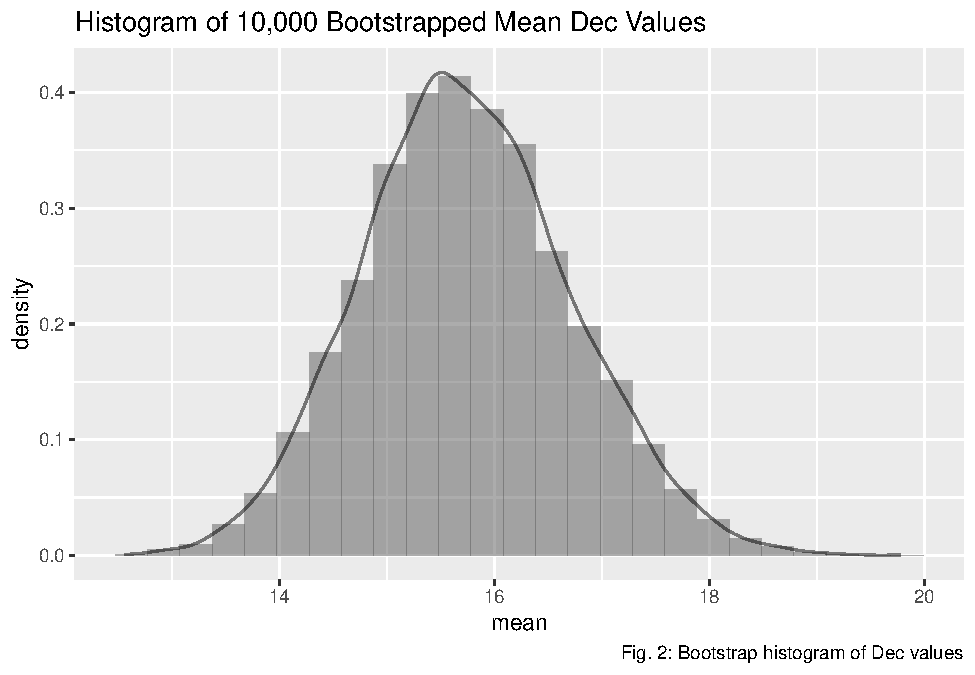
\includegraphics{paper_files/figure-latex/unnamed-chunk-1-1.pdf}

Next, we will perform the non-parametric bootstrap using 10,000
replications.

\begin{Shaded}
\begin{Highlighting}[]
\FunctionTok{set.seed}\NormalTok{(}\DecValTok{495}\NormalTok{)}
\NormalTok{orig\_mean }\OtherTok{\textless{}{-}} \FunctionTok{mean}\NormalTok{(}\SpecialCharTok{\textasciitilde{}}\NormalTok{ Dec, }\AttributeTok{data =}\NormalTok{ SnowGR) }\CommentTok{\# theta hat}

\FunctionTok{set.seed}\NormalTok{(}\DecValTok{495}\NormalTok{)}
\NormalTok{nboot }\OtherTok{\textless{}{-}} \DecValTok{10000}

\NormalTok{mean }\OtherTok{\textless{}{-}} \FunctionTok{rep}\NormalTok{(}\DecValTok{0}\NormalTok{,nboot)}
\NormalTok{sd }\OtherTok{\textless{}{-}} \FunctionTok{rep}\NormalTok{(}\DecValTok{0}\NormalTok{,nboot)}
\NormalTok{se }\OtherTok{\textless{}{-}} \FunctionTok{rep}\NormalTok{(}\DecValTok{0}\NormalTok{,nboot)}
\NormalTok{t\_stat }\OtherTok{\textless{}{-}} \FunctionTok{rep}\NormalTok{(}\DecValTok{0}\NormalTok{,nboot)}

\ControlFlowTok{for}\NormalTok{ (i }\ControlFlowTok{in} \DecValTok{1}\SpecialCharTok{:}\NormalTok{nboot) \{}
\NormalTok{  resampled }\OtherTok{\textless{}{-}} \FunctionTok{as.data.frame}\NormalTok{(mosaic}\SpecialCharTok{::}\FunctionTok{resample}\NormalTok{(SnowGR, }\AttributeTok{replace =} \ConstantTok{TRUE}\NormalTok{))}
\NormalTok{  mean[i] }\OtherTok{\textless{}{-}} \FunctionTok{mean}\NormalTok{(}\SpecialCharTok{\textasciitilde{}}\NormalTok{Dec, }\AttributeTok{data =}\NormalTok{ resampled)}
\NormalTok{  sd[i] }\OtherTok{\textless{}{-}} \FunctionTok{sd}\NormalTok{(}\SpecialCharTok{\textasciitilde{}}\NormalTok{Dec, }\AttributeTok{data =}\NormalTok{ resampled)}
\NormalTok{\}}

\NormalTok{dec\_means }\OtherTok{\textless{}{-}} \FunctionTok{as.data.frame}\NormalTok{(mean)}
\end{Highlighting}
\end{Shaded}

\begin{Shaded}
\begin{Highlighting}[]
\FunctionTok{gf\_dhistogram}\NormalTok{(}\SpecialCharTok{\textasciitilde{}}\NormalTok{ mean, }\AttributeTok{data =}\NormalTok{ dec\_means) }\SpecialCharTok{\%\textgreater{}\%}
  \FunctionTok{gf\_dens}\NormalTok{() }\SpecialCharTok{\%\textgreater{}\%}
  \FunctionTok{gf\_labs}\NormalTok{(}\AttributeTok{title =} \StringTok{"Histogram of 10,000 Bootstrapped Mean Dec Values"}\NormalTok{,}
          \AttributeTok{caption =} \StringTok{"Fig. 2: Bootstrap Histogram"}\NormalTok{)}
\end{Highlighting}
\end{Shaded}

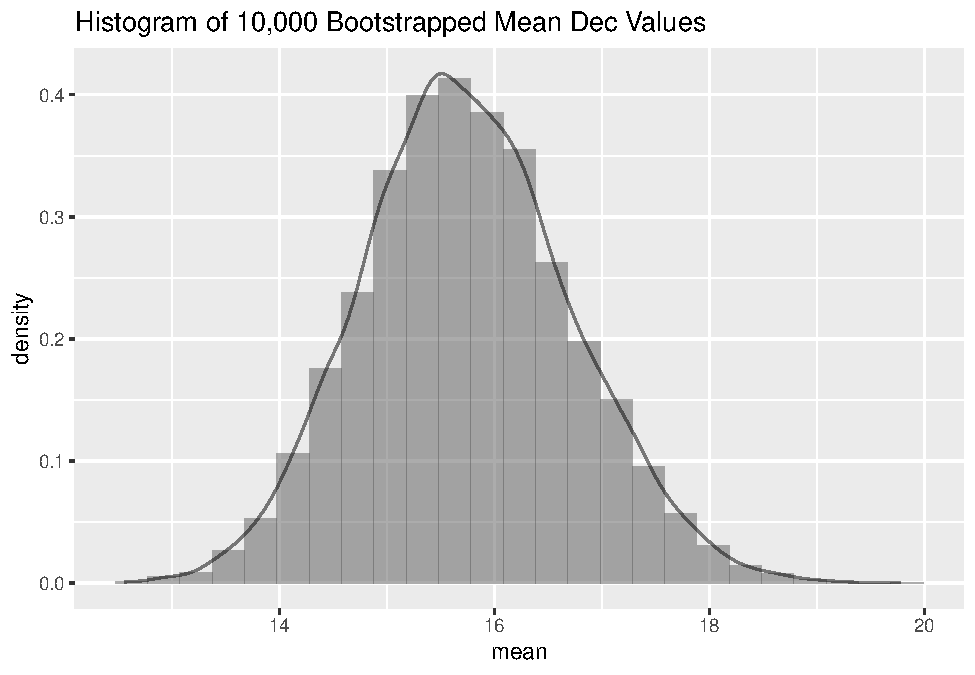
\includegraphics{paper_files/figure-latex/unnamed-chunk-3-1.pdf}

\hypertarget{standard-confidence-interval}{%
\subsection{Standard Confidence
Interval}\label{standard-confidence-interval}}

Confidence intervals are tools that are used to estimate a parameter.
Specifically, a confidence interval gives a range of values in which the
true value of the parameter may lie. An \(\alpha\)-level standard
confidence interval is given by
\[\hat{\theta}_S[\alpha] = \hat{\theta} \pm z_{\alpha}\hat{\sigma},\]
where \(\hat{\theta}\) is a point estimate of the parameter of interest
\(\theta\), \(\hat{\sigma}\) is the estimate of the standard deviation
of \(\hat{\theta}\) and \(z_{\alpha}\) is the \((100 *\alpha)\)th
percentile of the normal deviation \citep{Efron86}. We say that the
confidence interval constructed in this manner has a chance of capturing
the true parameter with a probability of \(\alpha\).

The standard confidence interval is built based on the assumption that
the distribution from which we are sampling is Normal. This means that
for an unknown distribution, the standard confidence interval could
present an incorrect range. However, the same process can be used with
bootstrap sampling to form the bootstrap percentile method. This means
that an approximate bootstrap confidence interval will be created in the
same automatic way that the standard confidence interval was created.
For bootstrapped confidence intervals, the number of bootstrap
replications \(B\) must be large (around 2000) due to the nature of
confidence intervals requiring greater accuracy \citep{Efron86}.

Using our example, to find a 95\% confidence interval for the population
mean of \texttt{Dec}, we would get the following:

\begin{Shaded}
\begin{Highlighting}[]
\FunctionTok{mean}\NormalTok{(}\SpecialCharTok{\textasciitilde{}}\NormalTok{ Dec, }\AttributeTok{data =}\NormalTok{ SnowGR) }\SpecialCharTok{+} \FunctionTok{qnorm}\NormalTok{(}\FunctionTok{c}\NormalTok{(}\FloatTok{0.025}\NormalTok{, }\FloatTok{0.975}\NormalTok{)) }\SpecialCharTok{*} 
  \FunctionTok{sd}\NormalTok{(}\SpecialCharTok{\textasciitilde{}}\NormalTok{ Dec, }\AttributeTok{data =}\NormalTok{ SnowGR)}\SpecialCharTok{/}\FunctionTok{sqrt}\NormalTok{(}\FunctionTok{nrow}\NormalTok{(SnowGR))}
\end{Highlighting}
\end{Shaded}

\begin{verbatim}
## [1] 13.85639 17.65957
\end{verbatim}

\begin{Shaded}
\begin{Highlighting}[]
\FunctionTok{gf\_histogram}\NormalTok{(}\SpecialCharTok{\textasciitilde{}}\NormalTok{ Dec, }\AttributeTok{data =}\NormalTok{ SnowGR) }\SpecialCharTok{+}
  \FunctionTok{labs}\NormalTok{(}\AttributeTok{x =} \StringTok{"Annual Snowfall in December"}\NormalTok{, }
       \AttributeTok{title =} \StringTok{"Distribution of Annual Snowfall in December"}\NormalTok{, }\AttributeTok{y =} \StringTok{"Count"}\NormalTok{,}
       \AttributeTok{caption =} \StringTok{"Fig. 3: Histogram with Standard Interval Shown"}\NormalTok{) }\SpecialCharTok{+}
  \FunctionTok{geom\_vline}\NormalTok{(}\FunctionTok{aes}\NormalTok{(}\AttributeTok{xintercept=} \FloatTok{13.85639}\NormalTok{)) }\SpecialCharTok{+}
  \FunctionTok{geom\_vline}\NormalTok{(}\FunctionTok{aes}\NormalTok{(}\AttributeTok{xintercept=} \FloatTok{17.65957}\NormalTok{))}
\end{Highlighting}
\end{Shaded}

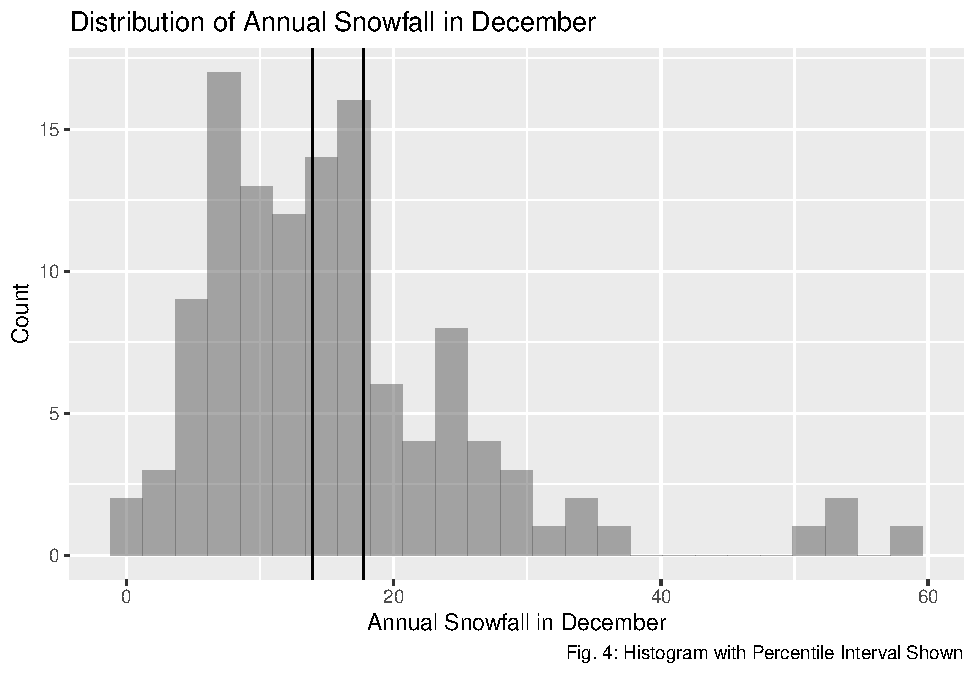
\includegraphics{paper_files/figure-latex/unnamed-chunk-5-1.pdf}

\hypertarget{the-percentile-method}{%
\subsection{The Percentile Method}\label{the-percentile-method}}

The percentile method interval is defined as the interval between the
\(100 * \alpha\) and the \(100(1 - \alpha)\) percentiles of the
bootstrap distribution of \(\hat{\theta}\). That is, the
\((1 - 2\alpha)\) coverage interval can be defined as
\([\hat{\theta}^*_\alpha,\hat{\theta}^*_{1-\alpha}]\)
\citep[\citet{EfronCasi}]{Efron86}. To go further, we can define
\(\hat{G}(t)\) as the bootstrap cdf, or the proportion of bootstrap
samples less than \(t\):
\[\hat{G}(t) = \frac{\#\{\hat{\theta^{*b} \leq t}\}}{B}.\] Thus the
\(\alpha\)th percentile point of the distribution is given by
\[\hat{\theta}_p[\alpha] = \hat{\theta^*_\alpha} = \hat{G}^{-1}(\alpha).\]
It follows that the percentile interval can be represented as
\[\left [ \hat{G}^{-1}(\alpha),\hat{G}^{-1}(1-\alpha) \right ].\] In the
case that the bootstrap distribution of
\(\hat{\theta}^* \sim N(\hat{\theta}, \hat{\sigma}^2)\), the
corresponding percentile interval would be equivalent to the standard
interval. However, this is not usually the case. When the bootstrap
distribution is non-normal, we can suppose that there exists, for all
\(\theta\), \[\hat{\phi} \sim N(\phi, \tau^2),\] for some monotone
transformation \(\hat{\phi} = g(\hat{\theta}), \phi = g(\theta)\), and
\(\tau\) is a constant. In other words, this transformation perfectly
normalizes the distribution of \(\hat{\theta}\). This transformation
invariant can be applied to the bootstrap replications such that
\[\hat{\phi}^{*b} = g\left( \hat{\theta}^{*b}\right ) \text{ for } b = 1,2,\dots, B.\]
The corresponding percentiles of the distribution transform similarly,
\(\hat{\phi}^*_\alpha = g \left ( \hat{\theta}^*_\alpha \right )\). Or
we can say that the \((1 - 2\alpha)\) percentile interval is
\(\hat{\phi} \pm \tau z_\alpha\) which can also be represented as
\([\hat{\phi}^*_\alpha,\hat{\phi}^*_{1-\alpha}]\). This means that the
interval on the \(\theta\) scale can be defined as
\[\hat{\theta}^*_\alpha = g^{-1}(\hat{\phi} \pm \tau z_\alpha).\] This
also can be represented as an interval,
\[\left [ g^{-1}(\hat{\phi} \pm \tau z_{1-\alpha}), g^{-1}(\hat{\phi} \pm \tau z_\alpha) \right ].\]
Therefore, the percentile method produces a correct interval for
\(\phi\) and due to the transformation invariance, also produces a
correct percentile interval for \(\theta\). This method assumes the
existence of some monotone normalizing mapping
\(\hat{\phi} = g(\hat{\theta}), \phi = g(\theta)\) and relies on that to
create a correct interval. Since the process is automatic, we do not
need to know the transformation itself, only that it exists. However, in
some cases, no monotone normalizing mapping will exist \citep{Efron86}.

Finding a 95\% confidence interval for the true population mean of
\texttt{Dec} using the percentile method, we get:

\begin{Shaded}
\begin{Highlighting}[]
\FunctionTok{qdata}\NormalTok{(}\SpecialCharTok{\textasciitilde{}}\NormalTok{ mean, }\FunctionTok{c}\NormalTok{(}\FloatTok{0.025}\NormalTok{, }\FloatTok{0.975}\NormalTok{), }\AttributeTok{data =}\NormalTok{ dec\_means)}
\end{Highlighting}
\end{Shaded}

\begin{verbatim}
##     2.5%    97.5% 
## 13.91170 17.72353
\end{verbatim}

\begin{Shaded}
\begin{Highlighting}[]
\FunctionTok{gf\_histogram}\NormalTok{(}\SpecialCharTok{\textasciitilde{}}\NormalTok{ Dec, }\AttributeTok{data =}\NormalTok{ SnowGR) }\SpecialCharTok{+}
  \FunctionTok{labs}\NormalTok{(}\AttributeTok{x =} \StringTok{"Annual Snowfall in December"}\NormalTok{, }
       \AttributeTok{title =} \StringTok{"Distribution of Annual Snowfall in December"}\NormalTok{, }\AttributeTok{y =} \StringTok{"Count"}\NormalTok{,}
       \AttributeTok{caption =} \StringTok{"Fig. 4: Histogram with Percentile Interval Shown"}\NormalTok{) }\SpecialCharTok{+}
  \FunctionTok{geom\_vline}\NormalTok{(}\FunctionTok{aes}\NormalTok{(}\AttributeTok{xintercept=} \FloatTok{13.91170}\NormalTok{)) }\SpecialCharTok{+}
  \FunctionTok{geom\_vline}\NormalTok{(}\FunctionTok{aes}\NormalTok{(}\AttributeTok{xintercept=} \FloatTok{17.72353}\NormalTok{))}
\end{Highlighting}
\end{Shaded}

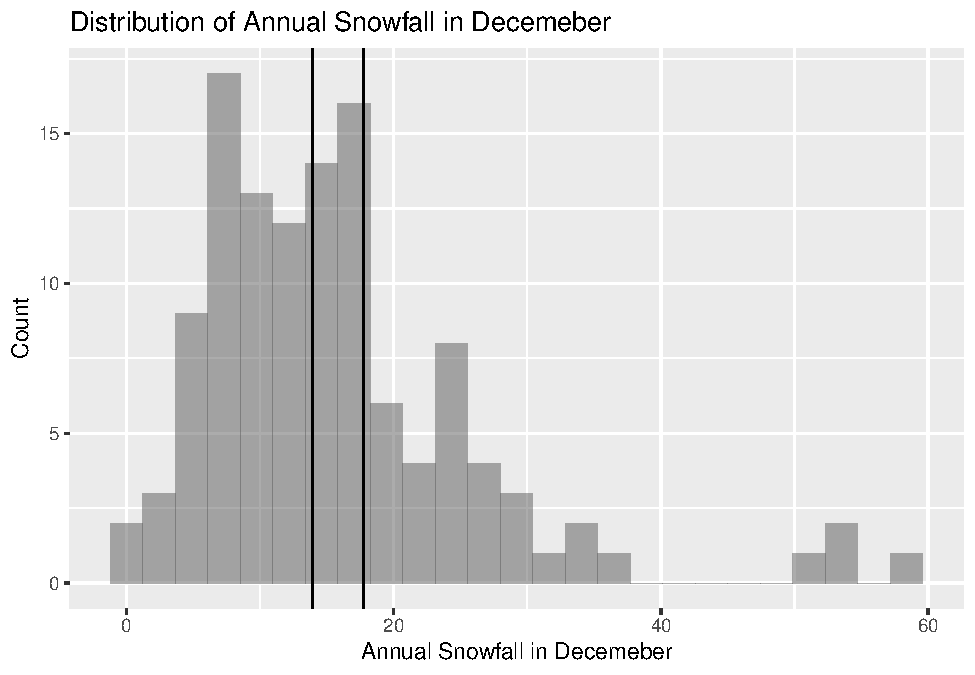
\includegraphics{paper_files/figure-latex/unnamed-chunk-7-1.pdf} This
interval is similar to the one created using the Standard method, but
shifted slightly to the right.

\hypertarget{the-bias-corrected-bc-method}{%
\subsection{The Bias-Corrected (BC)
Method}\label{the-bias-corrected-bc-method}}

The next method we will be looking at is the bias-corrected percentile
method (BC method) which is an improvement upon the previous percentile
method because we now take into account the possibility of bias. It can
be shown that \(\hat{\theta}\) is biased upwards relative to \(\theta\)
which means that the confidence intervals should be adjusted downwards
\citep[\citet{EfronCasi}]{Efron86}. From our simulated bootstrap
replications
\(\hat{\theta}^{*1}, \hat{\theta}^{*2}, \dots ,\hat{\theta}^{*B},\)
define \[p_0 = \frac{\#\{\hat{\theta^{*b} \leq \theta}\}}{B},\] and
define the bias-correction value \[z_0 = \Phi^{-1}(p_0),\] where
\(\Phi^{-1}\) is the inverse function of the standard normal cdf. Thus
we define a transformation
\(\hat{\phi} = g(\hat{\theta)}, \phi = g(\theta)\) such that for any
\(\theta\), \[\hat{\phi} \sim N(\phi - z_0\tau, \tau^2),\] with \(z_0\)
and \(\tau\) constants. This means that we can say the bias corrected
method has an \(\alpha\)-level endpoint can be represented as
\[\hat{\theta}_{BC}[\alpha] = \hat{G}^{-1} \left [ \Phi \left ( 2z_0 + z_\alpha\right ) \right ].\]
If \(\hat{G} = 0.50\), then half of the bootstrap distribution is less
than \(\hat{\theta}\) and our bias-correction value \(z_0 = 0\). In this
case, the confidence interval produced by BC would be the same interval
produced by the percentile method.

Using this method to create a 95\% confidence interval has a couple more
steps because we need to find the bias-correction value. First we
calculate the sample mean.

\begin{Shaded}
\begin{Highlighting}[]
\NormalTok{sample\_mean }\OtherTok{\textless{}{-}} \FunctionTok{mean}\NormalTok{(}\SpecialCharTok{\textasciitilde{}}\NormalTok{Dec, }\AttributeTok{data =}\NormalTok{ SnowGR); sample\_mean}
\end{Highlighting}
\end{Shaded}

\begin{verbatim}
## [1] 15.75798
\end{verbatim}

Then we find the proportion of bootstrap replications that have a sample
mean less than the original sample mean.

\begin{Shaded}
\begin{Highlighting}[]
\NormalTok{less\_than\_sample\_mean }\OtherTok{\textless{}{-}} \FunctionTok{sum}\NormalTok{(}\FunctionTok{ifelse}\NormalTok{(dec\_means }\SpecialCharTok{\textless{}=}\NormalTok{ sample\_mean, }\DecValTok{1}\NormalTok{, }\DecValTok{0}\NormalTok{))}\SpecialCharTok{/}\DecValTok{10000}
\NormalTok{less\_than\_sample\_mean}
\end{Highlighting}
\end{Shaded}

\begin{verbatim}
## [1] 0.5208
\end{verbatim}

From this, we can calculate the bias-correction value, \(z_0\):

\begin{Shaded}
\begin{Highlighting}[]
\NormalTok{z0 }\OtherTok{\textless{}{-}} \FunctionTok{qnorm}\NormalTok{(less\_than\_sample\_mean); z0}
\end{Highlighting}
\end{Shaded}

\begin{verbatim}
## [1] 0.05216151
\end{verbatim}

Then we can find the modified percentiles:

\begin{Shaded}
\begin{Highlighting}[]
\NormalTok{alphalow }\OtherTok{\textless{}{-}} \FloatTok{0.025}\NormalTok{; alphahigh }\OtherTok{\textless{}{-}} \FloatTok{0.975}

\NormalTok{newlow }\OtherTok{\textless{}{-}} \FunctionTok{pnorm}\NormalTok{(}\DecValTok{2}\SpecialCharTok{*}\NormalTok{z0 }\SpecialCharTok{+} \FunctionTok{qnorm}\NormalTok{(alphalow)); }\CommentTok{\#newlow}
\NormalTok{newhigh }\OtherTok{\textless{}{-}} \FunctionTok{pnorm}\NormalTok{(}\DecValTok{2}\SpecialCharTok{*}\NormalTok{z0 }\SpecialCharTok{+} \FunctionTok{qnorm}\NormalTok{(alphahigh)); }\CommentTok{\#newhigh}

\FunctionTok{qdata}\NormalTok{(}\SpecialCharTok{\textasciitilde{}}\NormalTok{ mean, }\FunctionTok{c}\NormalTok{(newlow, newhigh), }\AttributeTok{data =}\NormalTok{ dec\_means)}
\end{Highlighting}
\end{Shaded}

\begin{verbatim}
## 3.175238% 98.05047% 
##  14.01172  17.82017
\end{verbatim}

\begin{Shaded}
\begin{Highlighting}[]
\FunctionTok{gf\_histogram}\NormalTok{(}\SpecialCharTok{\textasciitilde{}}\NormalTok{ Dec, }\AttributeTok{data =}\NormalTok{ SnowGR) }\SpecialCharTok{+}
  \FunctionTok{labs}\NormalTok{(}\AttributeTok{x =} \StringTok{"Annual Snowfall in December"}\NormalTok{, }
       \AttributeTok{title =} \StringTok{"Distribution of Annual Snowfall in December"}\NormalTok{, }\AttributeTok{y =} \StringTok{"Count"}\NormalTok{,}
       \AttributeTok{caption =} \StringTok{"Fig. 5: Histogram with BC Interval Shown"}\NormalTok{) }\SpecialCharTok{+}
  \FunctionTok{geom\_vline}\NormalTok{(}\FunctionTok{aes}\NormalTok{(}\AttributeTok{xintercept=} \FloatTok{14.01172}\NormalTok{)) }\SpecialCharTok{+}
  \FunctionTok{geom\_vline}\NormalTok{(}\FunctionTok{aes}\NormalTok{(}\AttributeTok{xintercept=} \FloatTok{17.82017}\NormalTok{))}
\end{Highlighting}
\end{Shaded}

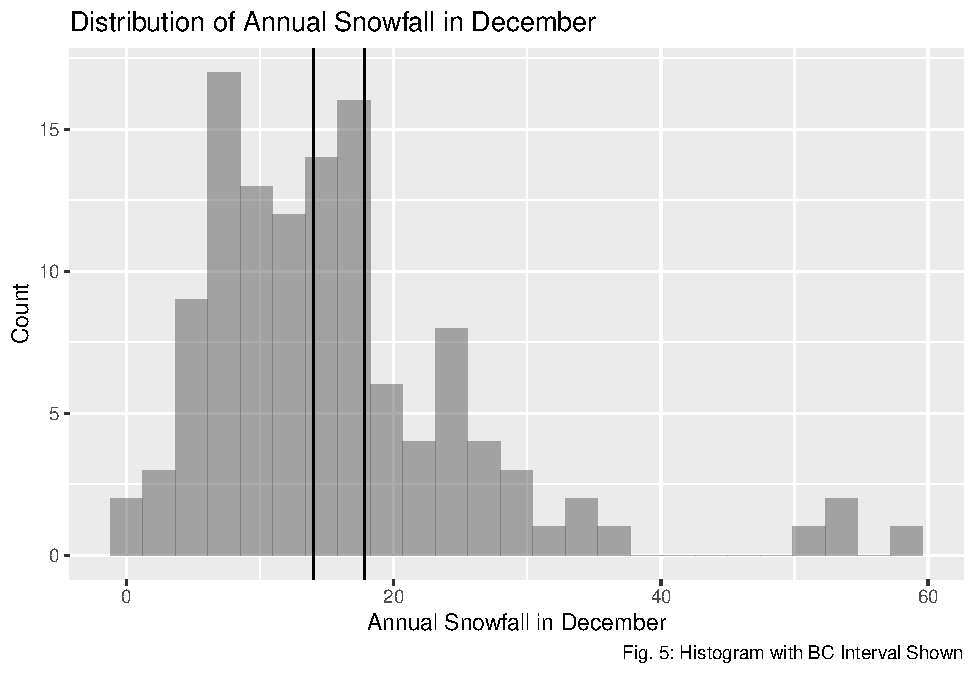
\includegraphics{paper_files/figure-latex/unnamed-chunk-12-1.pdf}

\hypertarget{the-bias-corrected-and-accelerated-bca-method}{%
\subsection{The Bias-Corrected and Accelerated (BCa)
Method}\label{the-bias-corrected-and-accelerated-bca-method}}

A further modification upon the BC interval is the bias corrected and
accelerated method (BCa). For this method, we do not assume the the
standard error, \(\tau\) is constant as we did in the BC interval
\citep[\citet{EfronCasi}]{Efron86}. Rather, we assume the existence of a
monotone transformation
\(\hat{\phi} = g(\hat{\theta)}, \phi = g(\theta)\) such that for any
\(\theta\),
\[\hat{\phi} \sim N(\phi - z_0\tau_\phi, \tau_\phi^2) \text{ where } \tau_\phi = 1+ a\phi.\]
The \(a\) is known as the acceleration and is a constant that describes
how the standard deviation of \(\hat{\phi}\) varies with \(\phi\). In
other words, \(a\) is proportional to the skewness of the bootstrap
distribution. For example, for one-parameter exponential families,
\(a=z_0\), however, there are many different algorithms to compute and
estimate \(a\) \citep{Flowers18}. Now, our \(\alpha\)-level endpoint
from BCa is
\[\hat{\theta}_{BCa}[\alpha] = \hat{G}^{-1} \left [ \Phi \left ( z_0 + \frac{z_0+z_\alpha}{1-a(z_0+z_a)} \right ) \right ].\]
If \(a = 0\), then
\(\hat{\theta}_{BCa}[\alpha] = \hat{\theta}_{BC}[\alpha].\) When
calculating a BCa interval, the acceleration value \(a\) is not a
function of the bootstrap distribution and must be calculated
separately, however the process is algorithmic and can be calculated
without too much work. Each of the three previous methods (percentile,
BC, and BCa) all build upon each other and have less restrictive
assumptions, however computation increases as we loosen assumptions.

In practice, we can use the jackknife procedure to estimate the
acceleration value for this method. Thus, we will run the jackknife
procedure:

\begin{Shaded}
\begin{Highlighting}[]
\NormalTok{theta }\OtherTok{\textless{}{-}} \ControlFlowTok{function}\NormalTok{(x)\{}\FunctionTok{mean}\NormalTok{(x)\}}
\NormalTok{jackknife\_results }\OtherTok{\textless{}{-}}\NormalTok{ bootstrap}\SpecialCharTok{::}\FunctionTok{jackknife}\NormalTok{(SnowGR}\SpecialCharTok{$}\NormalTok{Dec, theta) }
\end{Highlighting}
\end{Shaded}

We find the mean of the jackknife values below:

\begin{Shaded}
\begin{Highlighting}[]
\NormalTok{jackmean }\OtherTok{\textless{}{-}} \FunctionTok{mean}\NormalTok{(}\SpecialCharTok{\textasciitilde{}}\NormalTok{ jackknife\_results}\SpecialCharTok{$}\NormalTok{jack.values); jackmean}
\end{Highlighting}
\end{Shaded}

\begin{verbatim}
## [1] 15.75798
\end{verbatim}

Then we can compute \(a\).

\begin{Shaded}
\begin{Highlighting}[]
\NormalTok{estimated\_a }\OtherTok{\textless{}{-}}\NormalTok{ (}\DecValTok{1}\SpecialCharTok{/}\DecValTok{6}\NormalTok{)}\SpecialCharTok{*}\FunctionTok{sum}\NormalTok{((jackknife\_results}\SpecialCharTok{$}\NormalTok{jack.values }\SpecialCharTok{{-}}\NormalTok{ jackmean)}\SpecialCharTok{\^{}}\DecValTok{3}\NormalTok{)}\SpecialCharTok{/}
\NormalTok{  (}\FunctionTok{sum}\NormalTok{((jackknife\_results}\SpecialCharTok{$}\NormalTok{jack.values }\SpecialCharTok{{-}}\NormalTok{ jackmean)}\SpecialCharTok{\^{}}\DecValTok{2}\NormalTok{))}\SpecialCharTok{\^{}}\NormalTok{(}\FloatTok{1.5}\NormalTok{); estimated\_a}
\end{Highlighting}
\end{Shaded}

\begin{verbatim}
## [1] -0.02674911
\end{verbatim}

Now, we can find the adjust percentiles and the bias-corrected with
acceleration confidence interval.

\begin{Shaded}
\begin{Highlighting}[]
\NormalTok{a\_newlow }\OtherTok{\textless{}{-}} \FunctionTok{pnorm}\NormalTok{(z0 }\SpecialCharTok{+}\NormalTok{ (z0 }\SpecialCharTok{+} \FunctionTok{qnorm}\NormalTok{(alphalow))}\SpecialCharTok{/}
\NormalTok{                    (}\DecValTok{1}\SpecialCharTok{{-}}\NormalTok{estimated\_a}\SpecialCharTok{*}\NormalTok{(z0 }\SpecialCharTok{+} \FunctionTok{qnorm}\NormalTok{(alphalow)))); }\CommentTok{\#a\_newlow}
\NormalTok{a\_newhigh }\OtherTok{\textless{}{-}} \FunctionTok{pnorm}\NormalTok{(z0 }\SpecialCharTok{+}\NormalTok{ (z0 }\SpecialCharTok{+} \FunctionTok{qnorm}\NormalTok{(alphahigh))}\SpecialCharTok{/}
\NormalTok{                     (}\DecValTok{1}\SpecialCharTok{{-}}\NormalTok{estimated\_a}\SpecialCharTok{*}\NormalTok{(z0 }\SpecialCharTok{+} \FunctionTok{qnorm}\NormalTok{(alphahigh)))); }\CommentTok{\#a\_newhigh}
\FunctionTok{qdata}\NormalTok{(}\SpecialCharTok{\textasciitilde{}}\NormalTok{ mean, }\FunctionTok{c}\NormalTok{(a\_newlow, a\_newhigh), }\AttributeTok{data =}\NormalTok{ dec\_means)}
\end{Highlighting}
\end{Shaded}

\begin{verbatim}
## 2.510119% 97.50908% 
##  13.91591  17.72353
\end{verbatim}

\begin{Shaded}
\begin{Highlighting}[]
\FunctionTok{gf\_histogram}\NormalTok{(}\SpecialCharTok{\textasciitilde{}}\NormalTok{ Dec, }\AttributeTok{data =}\NormalTok{ SnowGR) }\SpecialCharTok{+}
  \FunctionTok{labs}\NormalTok{(}\AttributeTok{x =} \StringTok{"Annual Snowfall in December"}\NormalTok{, }
       \AttributeTok{title =} \StringTok{"Distribution of Annual Snowfall in December"}\NormalTok{, }\AttributeTok{y =} \StringTok{"Count"}\NormalTok{,}
       \AttributeTok{caption =} \StringTok{"Fig. 6: Histogram with BCa Interval Shown"}\NormalTok{) }\SpecialCharTok{+}
  \FunctionTok{geom\_vline}\NormalTok{(}\FunctionTok{aes}\NormalTok{(}\AttributeTok{xintercept=} \FloatTok{13.91591}\NormalTok{)) }\SpecialCharTok{+}
  \FunctionTok{geom\_vline}\NormalTok{(}\FunctionTok{aes}\NormalTok{(}\AttributeTok{xintercept=} \FloatTok{17.72353}\NormalTok{))}
\end{Highlighting}
\end{Shaded}

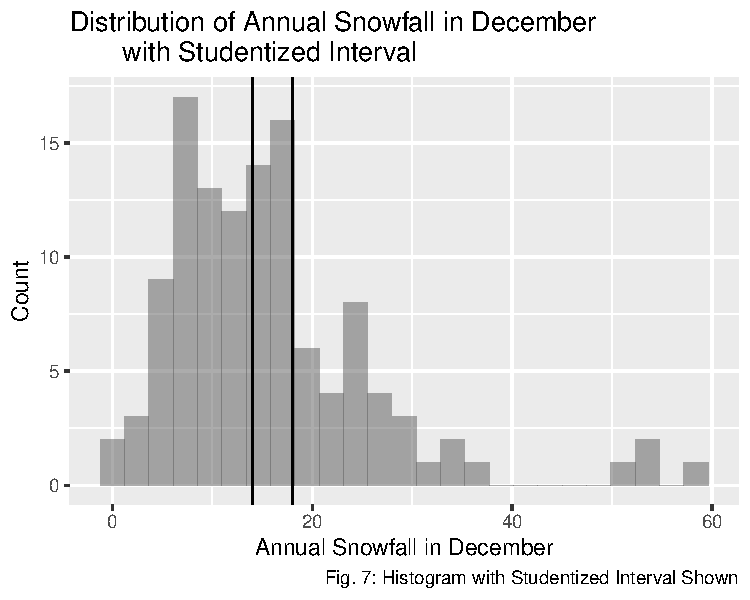
\includegraphics{paper_files/figure-latex/unnamed-chunk-17-1.pdf}

\hypertarget{the-bootstrap-t-studentized-method}{%
\subsection{The Bootstrap-t (Studentized)
Method}\label{the-bootstrap-t-studentized-method}}

The final method we explain is the bootstrap-t interval (or the
studentized method). Recall from earlier, our sample, \(X\) from which
we can calculate an estimate, \(\hat{\theta}(X)\) of the parameter of
interest \(\theta\) \citep[\citet{Puth15}]{Efron86}. We can also
estimate \(\hat{\sigma}(X)\) for the standard error of \(\theta\). We
can use these parameters to find the Student's \(t\)-statistic defined
as \[T = \frac{\hat{\theta} - \theta}{\hat{\sigma}}.\] As such, the
\(\alpha\)th percentile point of a confidence interval of \(\theta\)
would be \(\hat{\theta} - \hat{\sigma}T_{(\alpha)}\) where
\(T_{(\alpha)}\) represents the \(\alpha\)th percentile of the
\(t\)-distribution, \(T\). Unfortunately, the percentiles of the
t-distribution are unknown in most cases, but we can use bootstrapping
to estimate these percentiles. To do this, we perform a large number,
\(B\), of bootstrap samples, from which we can find the bootstrap
replications of the parameter of interest,
\(\hat{\theta^*} = \hat{\theta}(X^*)\), and the standard error,
\(\hat{\sigma^*} = \hat{\sigma}(X^*)\). From these we can calculate a
t-statistic for each bootstrap sample:
\[T^* = \frac{\hat{\theta}^* - \hat{\theta}}{\hat{\sigma}^*}.\] for each
bootstrap sample. Using a large number of these bootstrap samples, we
can estimate the percentiles of the \(t\)-distribution such that:
\[\hat{T}_{(\alpha)} = B*\alpha\text{th ordered value of all the bootstrap relications of }T^*.\]
This means that for \(B = 2000\) and \(\alpha = 0.90\), then
\(\hat{T}_{(\alpha)}\) is the 1,800th ordered point of all of the
bootstrap replications of \(T^*\). It follows that the \(\alpha\)th
studentized confidence interval endpoint can be given with
\[\hat{\theta}_T[\alpha] = \hat{\theta} - \hat{\sigma}T_{(\alpha)},\]
where we can estimate the standard error using
\[\hat{\sigma} = \frac{1-\hat{\theta}^2}{\sqrt{n}}.\] One of the main
factors why the studentized method is so popular is because we assume
that our bootstrapped statistic is pivotal which means that the
confidence interval does not depend on any other parameters. Instead, we
can calculate the appropriate confidence interval for the parameter of
interest specifically from the bootstrapped statistic
\citep[\citet{Puth15}]{Efron86}.

Following the process above, we can use the following to get our
studentized confidence interval \citep{Lau20}:

\begin{Shaded}
\begin{Highlighting}[]
\FunctionTok{set.seed}\NormalTok{(}\DecValTok{495}\NormalTok{)}

\NormalTok{orig\_mean }\OtherTok{\textless{}{-}} \FunctionTok{mean}\NormalTok{(}\SpecialCharTok{\textasciitilde{}}\NormalTok{ Dec, }\AttributeTok{data =}\NormalTok{ SnowGR) }\CommentTok{\# theta hat}
\NormalTok{orig\_se }\OtherTok{\textless{}{-}} \FunctionTok{sd}\NormalTok{(}\SpecialCharTok{\textasciitilde{}}\NormalTok{ Dec, }\AttributeTok{data =}\NormalTok{ SnowGR)}\SpecialCharTok{/}\FunctionTok{sqrt}\NormalTok{(}\FunctionTok{nrow}\NormalTok{(SnowGR))}

\NormalTok{se }\OtherTok{\textless{}{-}} \FunctionTok{rep}\NormalTok{(}\DecValTok{0}\NormalTok{,nboot)}
\NormalTok{t\_stat }\OtherTok{\textless{}{-}} \FunctionTok{rep}\NormalTok{(}\DecValTok{0}\NormalTok{,nboot)}

\ControlFlowTok{for}\NormalTok{ (i }\ControlFlowTok{in} \DecValTok{1}\SpecialCharTok{:}\NormalTok{nboot) \{}
\NormalTok{  se[i] }\OtherTok{\textless{}{-}}\NormalTok{ sd[i]}\SpecialCharTok{/}\FunctionTok{sqrt}\NormalTok{(}\FunctionTok{nrow}\NormalTok{(SnowGR))}
\NormalTok{  t\_stat[i] }\OtherTok{\textless{}{-}}\NormalTok{ (mean[i] }\SpecialCharTok{{-}}\NormalTok{ orig\_mean)}\SpecialCharTok{/}\NormalTok{se[i]}
\NormalTok{\}}

\NormalTok{dec\_t\_stat }\OtherTok{\textless{}{-}} \FunctionTok{as.data.frame}\NormalTok{(t\_stat)}

\NormalTok{q }\OtherTok{\textless{}{-}} \FunctionTok{unname}\NormalTok{(}\FunctionTok{quantile}\NormalTok{(dec\_t\_stat}\SpecialCharTok{$}\NormalTok{t\_stat, }\FunctionTok{c}\NormalTok{(}\FloatTok{0.025}\NormalTok{, }\FloatTok{0.975}\NormalTok{)))}
\NormalTok{lower }\OtherTok{\textless{}{-}}\NormalTok{ q[}\DecValTok{1}\NormalTok{]}
\NormalTok{upper }\OtherTok{\textless{}{-}}\NormalTok{ q[}\DecValTok{2}\NormalTok{]}

\FunctionTok{c}\NormalTok{(orig\_mean }\SpecialCharTok{{-}}\NormalTok{ upper}\SpecialCharTok{*}\NormalTok{orig\_se, orig\_mean }\SpecialCharTok{{-}}\NormalTok{ lower}\SpecialCharTok{*}\NormalTok{orig\_se)}
\end{Highlighting}
\end{Shaded}

\begin{verbatim}
## [1] 14.03467 18.01709
\end{verbatim}

This would give us the following histogram:

\begin{Shaded}
\begin{Highlighting}[]
\FunctionTok{gf\_histogram}\NormalTok{(}\SpecialCharTok{\textasciitilde{}}\NormalTok{ Dec, }\AttributeTok{data =}\NormalTok{ SnowGR) }\SpecialCharTok{+}
  \FunctionTok{labs}\NormalTok{(}\AttributeTok{x =} \StringTok{"Annual Snowfall in December"}\NormalTok{, }
       \AttributeTok{title =} \StringTok{"Distribution of Annual Snowfall in December"}\NormalTok{, }\AttributeTok{y =} \StringTok{"Count"}\NormalTok{, }
       \AttributeTok{caption =} \StringTok{"Fig. 7: Histogram with Studentized Interval Shown"}\NormalTok{) }\SpecialCharTok{+}
  \FunctionTok{geom\_vline}\NormalTok{(}\FunctionTok{aes}\NormalTok{(}\AttributeTok{xintercept=} \FloatTok{14.03467}\NormalTok{)) }\SpecialCharTok{+}
  \FunctionTok{geom\_vline}\NormalTok{(}\FunctionTok{aes}\NormalTok{(}\AttributeTok{xintercept=} \FloatTok{18.01709}\NormalTok{)) }
\end{Highlighting}
\end{Shaded}

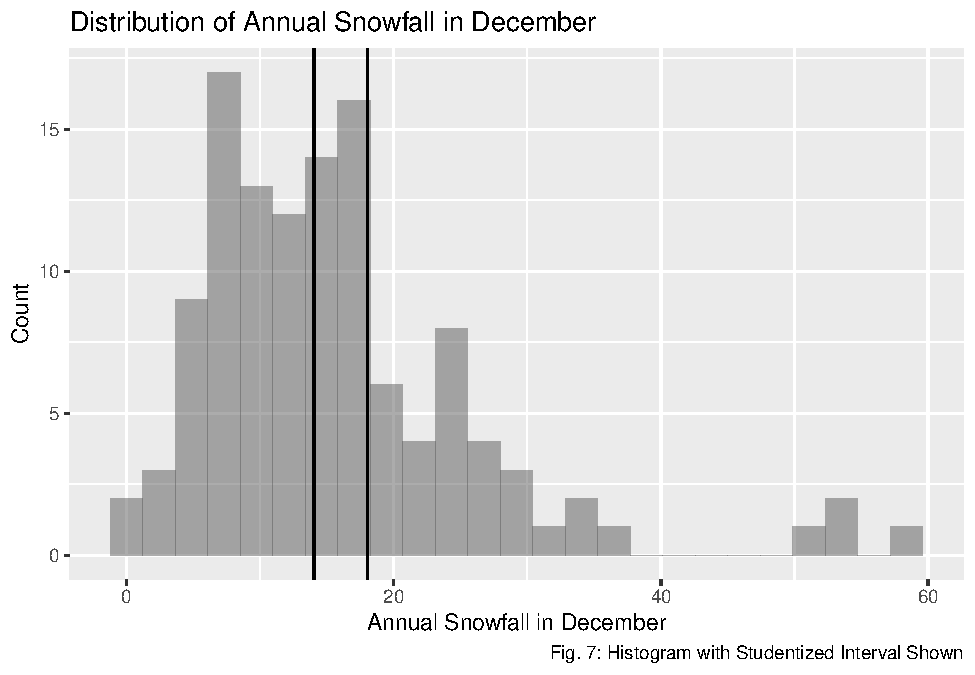
\includegraphics{paper_files/figure-latex/unnamed-chunk-19-1.pdf}

\hypertarget{simulation}{%
\section{Simulation}\label{simulation}}

For the simulation, we will randomly sample from distributions in which
we know the true population mean. For example, we will sampling from a
Gamma Distribution where we can find the true population mean using the
shape and rate parameters of the sample distribution. After we sample
from a distribution, we will create a bootstrapped confidence interval
for each of the methods we described in the exposition. Since we know
the true population mean of the distribution, we will determine if the
true population parameter is contained in the confidence interval for
each of the methods. We will perform this process a large number of
times (10,000) and then average by the number of iterations to determine
the average proportion that each bootstrapped confidence interval method
contains the true population mean. We will do this for a couple
different distributions as well as a range of sample sizes show how the
intervals perform with skewed distributions and larger sample sizes.

First, we create a function that calculates the bootstrapped confidence
intervals from a given sample. To do this, we first bootstrap the sample
and then perform each method.

Next, we will create the simulation that picks the random sample from a
distribution and tests to see if the sample creates bootstrapped
confidence intervals that contain the true population parameter. First,
we have the simulation of selecting from a Normal Distribution. Since we
have a \(N(0,1)\) distribution, out true population mean is 0.

Second, we select from a Gamma Distribution with a shape parameter of 1
and a scale parameter of 4. This means the true population parameter is
4.

After that, these functions will compile all of the information we have
created from the previous methods and run the simulations of each method
for a variety of sample sizes.

And here, we run the simulations for each of the distributions and store
the results.

Then, we can plot the results and compile the results into tables.

When we sample from the Gamma distribution which is a distribution that
is heavily skewed, the Studentized Confidence interval performs the
best. At a large sample size, the Studentized Confidence interval
contains the true population parameter about 94.5\% of the time. The
Studentized confidence interval outperforms the rest of the intervals by
a bit. The rest of the intervals are very similar to each other ranging
from a correct interval 92.5\% to 93\% of the time. In general, as the
sample size that we are bootstrapping from increases, the higher
percentage our confidence intervals predict correctly.

Similar to when we sampled from the Gamma distribution, the Studentized
confidence interval performed the best when we sampled from a Normal
distribution with around 95\% of the confidence intervals containing the
true population parameter. The next best is the Standard confidence
interval with a performance of around 94.5\% correct intervals at a high
sample size. The rest of the intervals performed similarly at around
94.2\% accuracy. As before, the accuracy increased as the sample size
increased.

\begin{Shaded}
\begin{Highlighting}[]
\FunctionTok{library}\NormalTok{(boot)}

\NormalTok{run\_sim\_log\_normal }\OtherTok{\textless{}{-}} \ControlFlowTok{function}\NormalTok{(sim\_reps) \{}
  \FunctionTok{set.seed}\NormalTok{(}\DecValTok{495}\NormalTok{)}
\NormalTok{  mean.fun }\OtherTok{\textless{}{-}} \ControlFlowTok{function}\NormalTok{(d, i) \{}
\NormalTok{    d }\OtherTok{\textless{}{-}}\NormalTok{ X[i]}
    \FunctionTok{return}\NormalTok{ (}\FunctionTok{c}\NormalTok{(}\FunctionTok{mean}\NormalTok{(d), }\FunctionTok{sd}\NormalTok{(d)))}
\NormalTok{  \}}
  
\NormalTok{  sample\_sizes }\OtherTok{\textless{}{-}} \FunctionTok{c}\NormalTok{(}\DecValTok{4}\NormalTok{, }\DecValTok{10}\NormalTok{, }\DecValTok{15}\NormalTok{, }\DecValTok{20}\NormalTok{, }\DecValTok{30}\NormalTok{, }\DecValTok{40}\NormalTok{, }\DecValTok{60}\NormalTok{, }\DecValTok{80}\NormalTok{, }\DecValTok{100}\NormalTok{)}
\NormalTok{  num\_sample\_sizes }\OtherTok{\textless{}{-}} \FunctionTok{length}\NormalTok{(sample\_sizes)}
\NormalTok{  master }\OtherTok{\textless{}{-}} \FunctionTok{matrix}\NormalTok{(}\AttributeTok{nrow =}\NormalTok{ num\_sample\_sizes, }\AttributeTok{ncol =} \DecValTok{6}\NormalTok{)}
  
  \ControlFlowTok{for}\NormalTok{(i }\ControlFlowTok{in} \DecValTok{1}\SpecialCharTok{:}\NormalTok{num\_sample\_sizes) \{}
  
\NormalTok{    norm\_contains }\OtherTok{\textless{}{-}} \FunctionTok{rep}\NormalTok{(}\DecValTok{0}\NormalTok{, sim\_reps)}
\NormalTok{    basic\_contains }\OtherTok{\textless{}{-}} \FunctionTok{rep}\NormalTok{(}\DecValTok{0}\NormalTok{, sim\_reps)}
\NormalTok{    student\_contains }\OtherTok{\textless{}{-}} \FunctionTok{rep}\NormalTok{(}\DecValTok{0}\NormalTok{, sim\_reps)}
\NormalTok{    percentile\_contains }\OtherTok{\textless{}{-}} \FunctionTok{rep}\NormalTok{(}\DecValTok{0}\NormalTok{, sim\_reps)}
\NormalTok{    bca\_contains }\OtherTok{\textless{}{-}} \FunctionTok{rep}\NormalTok{(}\DecValTok{0}\NormalTok{, sim\_reps)}
    
\NormalTok{    boot\_reps }\OtherTok{\textless{}{-}} \DecValTok{2000}
\NormalTok{    n }\OtherTok{\textless{}{-}}\NormalTok{ sample\_sizes[i]}
\NormalTok{    true\_mean }\OtherTok{\textless{}{-}} \FunctionTok{exp}\NormalTok{(}\DecValTok{1}\SpecialCharTok{/}\DecValTok{2}\NormalTok{)}
    
    \ControlFlowTok{for}\NormalTok{ (j }\ControlFlowTok{in} \DecValTok{1}\SpecialCharTok{:}\NormalTok{sim\_reps) \{}
\NormalTok{      X }\OtherTok{\textless{}{-}} \FunctionTok{rlnorm}\NormalTok{(n, }\DecValTok{0}\NormalTok{, }\DecValTok{1}\NormalTok{)}
\NormalTok{      values }\OtherTok{\textless{}{-}} \FunctionTok{data.frame}\NormalTok{(X)}
    
\NormalTok{      results }\OtherTok{\textless{}{-}} \FunctionTok{boot}\NormalTok{(}\AttributeTok{data =}\NormalTok{ values, }\AttributeTok{statistic =}\NormalTok{ mean.fun, }\AttributeTok{R =}\NormalTok{ boot\_reps)}
\NormalTok{      results}
      \CommentTok{\#plot(results)}
\NormalTok{      ci }\OtherTok{\textless{}{-}} \FunctionTok{boot.ci}\NormalTok{(results, }\AttributeTok{type =} \StringTok{"all"}\NormalTok{)}
      
\NormalTok{      norm\_contains[j] }\OtherTok{\textless{}{-}}\NormalTok{ true\_mean }\SpecialCharTok{\textgreater{}=}\NormalTok{ ci}\SpecialCharTok{$}\NormalTok{normal[}\DecValTok{2}\NormalTok{] }\SpecialCharTok{\&}\NormalTok{ true\_mean }\SpecialCharTok{\textless{}=}\NormalTok{ ci}\SpecialCharTok{$}\NormalTok{normal[}\DecValTok{3}\NormalTok{]}
\NormalTok{      basic\_contains[j] }\OtherTok{\textless{}{-}}\NormalTok{ true\_mean }\SpecialCharTok{\textgreater{}=}\NormalTok{ ci}\SpecialCharTok{$}\NormalTok{basic[}\DecValTok{4}\NormalTok{] }\SpecialCharTok{\&}\NormalTok{ true\_mean }\SpecialCharTok{\textless{}=}\NormalTok{ ci}\SpecialCharTok{$}\NormalTok{basic[}\DecValTok{5}\NormalTok{]}
\NormalTok{      student\_contains[j] }\OtherTok{\textless{}{-}}\NormalTok{ true\_mean }\SpecialCharTok{\textgreater{}=}\NormalTok{ ci}\SpecialCharTok{$}\NormalTok{student[}\DecValTok{4}\NormalTok{] }\SpecialCharTok{\&}\NormalTok{ true\_mean }\SpecialCharTok{\textless{}=}\NormalTok{ ci}\SpecialCharTok{$}\NormalTok{student[}\DecValTok{5}\NormalTok{]}
\NormalTok{      percentile\_contains[j] }\OtherTok{\textless{}{-}}\NormalTok{ true\_mean }\SpecialCharTok{\textgreater{}=}\NormalTok{ ci}\SpecialCharTok{$}\NormalTok{percent[}\DecValTok{4}\NormalTok{] }\SpecialCharTok{\&}\NormalTok{ true\_mean }\SpecialCharTok{\textless{}=}\NormalTok{ ci}\SpecialCharTok{$}\NormalTok{percent[}\DecValTok{5}\NormalTok{]}
\NormalTok{      bca\_contains[j] }\OtherTok{\textless{}{-}}\NormalTok{ true\_mean }\SpecialCharTok{\textgreater{}=}\NormalTok{ ci}\SpecialCharTok{$}\NormalTok{bca[}\DecValTok{4}\NormalTok{] }\SpecialCharTok{\&}\NormalTok{ true\_mean }\SpecialCharTok{\textless{}=}\NormalTok{ ci}\SpecialCharTok{$}\NormalTok{bca[}\DecValTok{5}\NormalTok{]}
      
\NormalTok{    \}}
    
\NormalTok{    master[i, }\DecValTok{1}\NormalTok{] }\OtherTok{\textless{}{-}}\NormalTok{ sample\_sizes[i]}
\NormalTok{    master[i, }\DecValTok{2}\NormalTok{] }\OtherTok{\textless{}{-}} \FunctionTok{sum}\NormalTok{(norm\_contains)}\SpecialCharTok{/}\NormalTok{sim\_reps}
\NormalTok{    master[i, }\DecValTok{3}\NormalTok{] }\OtherTok{\textless{}{-}} \FunctionTok{sum}\NormalTok{(basic\_contains)}\SpecialCharTok{/}\NormalTok{sim\_reps}
\NormalTok{    master[i, }\DecValTok{4}\NormalTok{] }\OtherTok{\textless{}{-}} \FunctionTok{sum}\NormalTok{(student\_contains)}\SpecialCharTok{/}\NormalTok{sim\_reps}
\NormalTok{    master[i, }\DecValTok{5}\NormalTok{] }\OtherTok{\textless{}{-}} \FunctionTok{sum}\NormalTok{(percentile\_contains)}\SpecialCharTok{/}\NormalTok{sim\_reps}
\NormalTok{    master[i, }\DecValTok{6}\NormalTok{] }\OtherTok{\textless{}{-}} \FunctionTok{sum}\NormalTok{(bca\_contains)}\SpecialCharTok{/}\NormalTok{sim\_reps}
\NormalTok{  \}}
  
\NormalTok{  master\_df }\OtherTok{\textless{}{-}} \FunctionTok{as.data.frame}\NormalTok{(master) }\SpecialCharTok{\%\textgreater{}\%} 
      \FunctionTok{rename}\NormalTok{(}\StringTok{"Sample\_Size"} \OtherTok{=}\NormalTok{ V1, }\StringTok{"Normal"} \OtherTok{=}\NormalTok{ V2, }\StringTok{"Basic"} \OtherTok{=}\NormalTok{ V3, }\StringTok{"Studentized"} \OtherTok{=}\NormalTok{ V4, }
             \StringTok{"Percentile"} \OtherTok{=}\NormalTok{ V5, }\StringTok{"BCa"} \OtherTok{=}\NormalTok{ V6) }
\NormalTok{  master\_df}
\NormalTok{\}}
\end{Highlighting}
\end{Shaded}

\begin{Shaded}
\begin{Highlighting}[]
\FunctionTok{library}\NormalTok{(boot)}

\NormalTok{run\_sim\_normal }\OtherTok{\textless{}{-}} \ControlFlowTok{function}\NormalTok{(sim\_reps) \{}
  \FunctionTok{set.seed}\NormalTok{(}\DecValTok{495}\NormalTok{)}
\NormalTok{  mean.fun }\OtherTok{\textless{}{-}} \ControlFlowTok{function}\NormalTok{(d, i) \{}
\NormalTok{    d }\OtherTok{\textless{}{-}}\NormalTok{ X[i]}
    \FunctionTok{return}\NormalTok{ (}\FunctionTok{c}\NormalTok{(}\FunctionTok{mean}\NormalTok{(d), }\FunctionTok{sd}\NormalTok{(d)))}
\NormalTok{  \}}
  
\NormalTok{  sample\_sizes }\OtherTok{\textless{}{-}} \FunctionTok{c}\NormalTok{(}\DecValTok{4}\NormalTok{, }\DecValTok{10}\NormalTok{, }\DecValTok{15}\NormalTok{, }\DecValTok{20}\NormalTok{, }\DecValTok{30}\NormalTok{, }\DecValTok{40}\NormalTok{, }\DecValTok{60}\NormalTok{, }\DecValTok{80}\NormalTok{, }\DecValTok{100}\NormalTok{)}
\NormalTok{  num\_sample\_sizes }\OtherTok{\textless{}{-}} \FunctionTok{length}\NormalTok{(sample\_sizes)}
\NormalTok{  master }\OtherTok{\textless{}{-}} \FunctionTok{matrix}\NormalTok{(}\AttributeTok{nrow =}\NormalTok{ num\_sample\_sizes, }\AttributeTok{ncol =} \DecValTok{6}\NormalTok{)}
  
  \ControlFlowTok{for}\NormalTok{(i }\ControlFlowTok{in} \DecValTok{1}\SpecialCharTok{:}\NormalTok{num\_sample\_sizes) \{}
  
\NormalTok{    norm\_contains }\OtherTok{\textless{}{-}} \FunctionTok{rep}\NormalTok{(}\DecValTok{0}\NormalTok{, sim\_reps)}
\NormalTok{    basic\_contains }\OtherTok{\textless{}{-}} \FunctionTok{rep}\NormalTok{(}\DecValTok{0}\NormalTok{, sim\_reps)}
\NormalTok{    student\_contains }\OtherTok{\textless{}{-}} \FunctionTok{rep}\NormalTok{(}\DecValTok{0}\NormalTok{, sim\_reps)}
\NormalTok{    percentile\_contains }\OtherTok{\textless{}{-}} \FunctionTok{rep}\NormalTok{(}\DecValTok{0}\NormalTok{, sim\_reps)}
\NormalTok{    bca\_contains }\OtherTok{\textless{}{-}} \FunctionTok{rep}\NormalTok{(}\DecValTok{0}\NormalTok{, sim\_reps)}
    
\NormalTok{    boot\_reps }\OtherTok{\textless{}{-}} \DecValTok{2000}
\NormalTok{    n }\OtherTok{\textless{}{-}}\NormalTok{ sample\_sizes[i]}
\NormalTok{    true\_mean }\OtherTok{\textless{}{-}} \DecValTok{0}
    
    \ControlFlowTok{for}\NormalTok{ (j }\ControlFlowTok{in} \DecValTok{1}\SpecialCharTok{:}\NormalTok{sim\_reps) \{}
\NormalTok{      X }\OtherTok{\textless{}{-}} \FunctionTok{rnorm}\NormalTok{(n, }\DecValTok{0}\NormalTok{, }\DecValTok{1}\NormalTok{)}
\NormalTok{      values }\OtherTok{\textless{}{-}} \FunctionTok{data.frame}\NormalTok{(X)}
    
\NormalTok{      results }\OtherTok{\textless{}{-}} \FunctionTok{boot}\NormalTok{(}\AttributeTok{data =}\NormalTok{ values, }\AttributeTok{statistic =}\NormalTok{ mean.fun, }\AttributeTok{R =}\NormalTok{ boot\_reps)}
\NormalTok{      results}
      \CommentTok{\#plot(results)}
\NormalTok{      ci }\OtherTok{\textless{}{-}} \FunctionTok{boot.ci}\NormalTok{(results, }\AttributeTok{type =} \StringTok{"all"}\NormalTok{)}
      
\NormalTok{      norm\_contains[j] }\OtherTok{\textless{}{-}}\NormalTok{ true\_mean }\SpecialCharTok{\textgreater{}=}\NormalTok{ ci}\SpecialCharTok{$}\NormalTok{normal[}\DecValTok{2}\NormalTok{] }\SpecialCharTok{\&}\NormalTok{ true\_mean }\SpecialCharTok{\textless{}=}\NormalTok{ ci}\SpecialCharTok{$}\NormalTok{normal[}\DecValTok{3}\NormalTok{]}
\NormalTok{      basic\_contains[j] }\OtherTok{\textless{}{-}}\NormalTok{ true\_mean }\SpecialCharTok{\textgreater{}=}\NormalTok{ ci}\SpecialCharTok{$}\NormalTok{basic[}\DecValTok{4}\NormalTok{] }\SpecialCharTok{\&}\NormalTok{ true\_mean }\SpecialCharTok{\textless{}=}\NormalTok{ ci}\SpecialCharTok{$}\NormalTok{basic[}\DecValTok{5}\NormalTok{]}
\NormalTok{      student\_contains[j] }\OtherTok{\textless{}{-}}\NormalTok{ true\_mean }\SpecialCharTok{\textgreater{}=}\NormalTok{ ci}\SpecialCharTok{$}\NormalTok{student[}\DecValTok{4}\NormalTok{] }\SpecialCharTok{\&}\NormalTok{ true\_mean }\SpecialCharTok{\textless{}=}\NormalTok{ ci}\SpecialCharTok{$}\NormalTok{student[}\DecValTok{5}\NormalTok{]}
\NormalTok{      percentile\_contains[j] }\OtherTok{\textless{}{-}}\NormalTok{ true\_mean }\SpecialCharTok{\textgreater{}=}\NormalTok{ ci}\SpecialCharTok{$}\NormalTok{percent[}\DecValTok{4}\NormalTok{] }\SpecialCharTok{\&}\NormalTok{ true\_mean }\SpecialCharTok{\textless{}=}\NormalTok{ ci}\SpecialCharTok{$}\NormalTok{percent[}\DecValTok{5}\NormalTok{]}
\NormalTok{      bca\_contains[j] }\OtherTok{\textless{}{-}}\NormalTok{ true\_mean }\SpecialCharTok{\textgreater{}=}\NormalTok{ ci}\SpecialCharTok{$}\NormalTok{bca[}\DecValTok{4}\NormalTok{] }\SpecialCharTok{\&}\NormalTok{ true\_mean }\SpecialCharTok{\textless{}=}\NormalTok{ ci}\SpecialCharTok{$}\NormalTok{bca[}\DecValTok{5}\NormalTok{]}
      
\NormalTok{    \}}
    
\NormalTok{    master[i, }\DecValTok{1}\NormalTok{] }\OtherTok{\textless{}{-}}\NormalTok{ sample\_sizes[i]}
\NormalTok{    master[i, }\DecValTok{2}\NormalTok{] }\OtherTok{\textless{}{-}} \FunctionTok{sum}\NormalTok{(norm\_contains)}\SpecialCharTok{/}\NormalTok{sim\_reps}
\NormalTok{    master[i, }\DecValTok{3}\NormalTok{] }\OtherTok{\textless{}{-}} \FunctionTok{sum}\NormalTok{(basic\_contains)}\SpecialCharTok{/}\NormalTok{sim\_reps}
\NormalTok{    master[i, }\DecValTok{4}\NormalTok{] }\OtherTok{\textless{}{-}} \FunctionTok{sum}\NormalTok{(student\_contains)}\SpecialCharTok{/}\NormalTok{sim\_reps}
\NormalTok{    master[i, }\DecValTok{5}\NormalTok{] }\OtherTok{\textless{}{-}} \FunctionTok{sum}\NormalTok{(percentile\_contains)}\SpecialCharTok{/}\NormalTok{sim\_reps}
\NormalTok{    master[i, }\DecValTok{6}\NormalTok{] }\OtherTok{\textless{}{-}} \FunctionTok{sum}\NormalTok{(bca\_contains)}\SpecialCharTok{/}\NormalTok{sim\_reps}
\NormalTok{  \}}
  
\NormalTok{  master\_df }\OtherTok{\textless{}{-}} \FunctionTok{as.data.frame}\NormalTok{(master) }\SpecialCharTok{\%\textgreater{}\%} 
      \FunctionTok{rename}\NormalTok{(}\StringTok{"Sample\_Size"} \OtherTok{=}\NormalTok{ V1, }\StringTok{"Normal"} \OtherTok{=}\NormalTok{ V2, }\StringTok{"Basic"} \OtherTok{=}\NormalTok{ V3, }\StringTok{"Studentized"} \OtherTok{=}\NormalTok{ V4, }
             \StringTok{"Percentile"} \OtherTok{=}\NormalTok{ V5, }\StringTok{"BCa"} \OtherTok{=}\NormalTok{ V6) }
\NormalTok{  master\_df}
\NormalTok{\}}
\end{Highlighting}
\end{Shaded}

\begin{Shaded}
\begin{Highlighting}[]
\FunctionTok{library}\NormalTok{(boot)}

\NormalTok{run\_sim\_gamma }\OtherTok{\textless{}{-}} \ControlFlowTok{function}\NormalTok{(sim\_reps) \{}
  \FunctionTok{set.seed}\NormalTok{(}\DecValTok{495}\NormalTok{)}
\NormalTok{  mean.fun }\OtherTok{\textless{}{-}} \ControlFlowTok{function}\NormalTok{(d, i) \{}
\NormalTok{    d }\OtherTok{\textless{}{-}}\NormalTok{ X[i]}
    \FunctionTok{return}\NormalTok{ (}\FunctionTok{c}\NormalTok{(}\FunctionTok{mean}\NormalTok{(d), }\FunctionTok{sd}\NormalTok{(d)))}
\NormalTok{  \}}
  
\NormalTok{  sample\_sizes }\OtherTok{\textless{}{-}} \FunctionTok{c}\NormalTok{(}\DecValTok{4}\NormalTok{, }\DecValTok{10}\NormalTok{, }\DecValTok{15}\NormalTok{, }\DecValTok{20}\NormalTok{, }\DecValTok{30}\NormalTok{, }\DecValTok{40}\NormalTok{, }\DecValTok{60}\NormalTok{, }\DecValTok{80}\NormalTok{, }\DecValTok{100}\NormalTok{)}
\NormalTok{  num\_sample\_sizes }\OtherTok{\textless{}{-}} \FunctionTok{length}\NormalTok{(sample\_sizes)}
\NormalTok{  master }\OtherTok{\textless{}{-}} \FunctionTok{matrix}\NormalTok{(}\AttributeTok{nrow =}\NormalTok{ num\_sample\_sizes, }\AttributeTok{ncol =} \DecValTok{6}\NormalTok{)}
  
  \ControlFlowTok{for}\NormalTok{(i }\ControlFlowTok{in} \DecValTok{1}\SpecialCharTok{:}\NormalTok{num\_sample\_sizes) \{}
  
\NormalTok{    norm\_contains }\OtherTok{\textless{}{-}} \FunctionTok{rep}\NormalTok{(}\DecValTok{0}\NormalTok{, sim\_reps)}
\NormalTok{    basic\_contains }\OtherTok{\textless{}{-}} \FunctionTok{rep}\NormalTok{(}\DecValTok{0}\NormalTok{, sim\_reps)}
\NormalTok{    student\_contains }\OtherTok{\textless{}{-}} \FunctionTok{rep}\NormalTok{(}\DecValTok{0}\NormalTok{, sim\_reps)}
\NormalTok{    percentile\_contains }\OtherTok{\textless{}{-}} \FunctionTok{rep}\NormalTok{(}\DecValTok{0}\NormalTok{, sim\_reps)}
\NormalTok{    bca\_contains }\OtherTok{\textless{}{-}} \FunctionTok{rep}\NormalTok{(}\DecValTok{0}\NormalTok{, sim\_reps)}
    
\NormalTok{    boot\_reps }\OtherTok{\textless{}{-}} \DecValTok{2000}
\NormalTok{    n }\OtherTok{\textless{}{-}}\NormalTok{ sample\_sizes[i]}
\NormalTok{    true\_mean }\OtherTok{\textless{}{-}} \DecValTok{4}
    
    \ControlFlowTok{for}\NormalTok{ (j }\ControlFlowTok{in} \DecValTok{1}\SpecialCharTok{:}\NormalTok{sim\_reps) \{}
\NormalTok{      X }\OtherTok{\textless{}{-}} \FunctionTok{rgamma}\NormalTok{(sample\_sizes, }\AttributeTok{shape =} \DecValTok{1}\NormalTok{, }\AttributeTok{scale =} \DecValTok{4}\NormalTok{)}
\NormalTok{      values }\OtherTok{\textless{}{-}} \FunctionTok{data.frame}\NormalTok{(X)}
    
\NormalTok{      results }\OtherTok{\textless{}{-}} \FunctionTok{boot}\NormalTok{(}\AttributeTok{data =}\NormalTok{ values, }\AttributeTok{statistic =}\NormalTok{ mean.fun, }\AttributeTok{R =}\NormalTok{ boot\_reps)}
\NormalTok{      results}
      \CommentTok{\#plot(results)}
\NormalTok{      ci }\OtherTok{\textless{}{-}} \FunctionTok{boot.ci}\NormalTok{(results, }\AttributeTok{type =} \StringTok{"all"}\NormalTok{)}
      
\NormalTok{      norm\_contains[j] }\OtherTok{\textless{}{-}}\NormalTok{ true\_mean }\SpecialCharTok{\textgreater{}=}\NormalTok{ ci}\SpecialCharTok{$}\NormalTok{normal[}\DecValTok{2}\NormalTok{] }\SpecialCharTok{\&}\NormalTok{ true\_mean }\SpecialCharTok{\textless{}=}\NormalTok{ ci}\SpecialCharTok{$}\NormalTok{normal[}\DecValTok{3}\NormalTok{]}
\NormalTok{      basic\_contains[j] }\OtherTok{\textless{}{-}}\NormalTok{ true\_mean }\SpecialCharTok{\textgreater{}=}\NormalTok{ ci}\SpecialCharTok{$}\NormalTok{basic[}\DecValTok{4}\NormalTok{] }\SpecialCharTok{\&}\NormalTok{ true\_mean }\SpecialCharTok{\textless{}=}\NormalTok{ ci}\SpecialCharTok{$}\NormalTok{basic[}\DecValTok{5}\NormalTok{]}
\NormalTok{      student\_contains[j] }\OtherTok{\textless{}{-}}\NormalTok{ true\_mean }\SpecialCharTok{\textgreater{}=}\NormalTok{ ci}\SpecialCharTok{$}\NormalTok{student[}\DecValTok{4}\NormalTok{] }\SpecialCharTok{\&}\NormalTok{ true\_mean }\SpecialCharTok{\textless{}=}\NormalTok{ ci}\SpecialCharTok{$}\NormalTok{student[}\DecValTok{5}\NormalTok{]}
\NormalTok{      percentile\_contains[j] }\OtherTok{\textless{}{-}}\NormalTok{ true\_mean }\SpecialCharTok{\textgreater{}=}\NormalTok{ ci}\SpecialCharTok{$}\NormalTok{percent[}\DecValTok{4}\NormalTok{] }\SpecialCharTok{\&}\NormalTok{ true\_mean }\SpecialCharTok{\textless{}=}\NormalTok{ ci}\SpecialCharTok{$}\NormalTok{percent[}\DecValTok{5}\NormalTok{]}
\NormalTok{      bca\_contains[j] }\OtherTok{\textless{}{-}}\NormalTok{ true\_mean }\SpecialCharTok{\textgreater{}=}\NormalTok{ ci}\SpecialCharTok{$}\NormalTok{bca[}\DecValTok{4}\NormalTok{] }\SpecialCharTok{\&}\NormalTok{ true\_mean }\SpecialCharTok{\textless{}=}\NormalTok{ ci}\SpecialCharTok{$}\NormalTok{bca[}\DecValTok{5}\NormalTok{]}
      
\NormalTok{    \}}
    
\NormalTok{    master[i, }\DecValTok{1}\NormalTok{] }\OtherTok{\textless{}{-}}\NormalTok{ sample\_sizes[i]}
\NormalTok{    master[i, }\DecValTok{2}\NormalTok{] }\OtherTok{\textless{}{-}} \FunctionTok{sum}\NormalTok{(norm\_contains)}\SpecialCharTok{/}\NormalTok{sim\_reps}
\NormalTok{    master[i, }\DecValTok{3}\NormalTok{] }\OtherTok{\textless{}{-}} \FunctionTok{sum}\NormalTok{(basic\_contains)}\SpecialCharTok{/}\NormalTok{sim\_reps}
\NormalTok{    master[i, }\DecValTok{4}\NormalTok{] }\OtherTok{\textless{}{-}} \FunctionTok{sum}\NormalTok{(student\_contains)}\SpecialCharTok{/}\NormalTok{sim\_reps}
\NormalTok{    master[i, }\DecValTok{5}\NormalTok{] }\OtherTok{\textless{}{-}} \FunctionTok{sum}\NormalTok{(percentile\_contains)}\SpecialCharTok{/}\NormalTok{sim\_reps}
\NormalTok{    master[i, }\DecValTok{6}\NormalTok{] }\OtherTok{\textless{}{-}} \FunctionTok{sum}\NormalTok{(bca\_contains)}\SpecialCharTok{/}\NormalTok{sim\_reps}
\NormalTok{  \}}
  
\NormalTok{  master\_df }\OtherTok{\textless{}{-}} \FunctionTok{as.data.frame}\NormalTok{(master) }\SpecialCharTok{\%\textgreater{}\%} 
      \FunctionTok{rename}\NormalTok{(}\StringTok{"Sample\_Size"} \OtherTok{=}\NormalTok{ V1, }\StringTok{"Normal"} \OtherTok{=}\NormalTok{ V2, }\StringTok{"Basic"} \OtherTok{=}\NormalTok{ V3, }\StringTok{"Studentized"} \OtherTok{=}\NormalTok{ V4, }
             \StringTok{"Percentile"} \OtherTok{=}\NormalTok{ V5, }\StringTok{"BCa"} \OtherTok{=}\NormalTok{ V6) }
\NormalTok{  master\_df}
\NormalTok{\}}
\end{Highlighting}
\end{Shaded}

\begin{Shaded}
\begin{Highlighting}[]
\FunctionTok{set.seed}\NormalTok{(}\DecValTok{495}\NormalTok{)}
\NormalTok{log\_normal\_df }\OtherTok{\textless{}{-}} \FunctionTok{run\_sim\_log\_normal}\NormalTok{(}\DecValTok{10000}\NormalTok{)}
\FunctionTok{write.csv}\NormalTok{(log\_normal\_df,}\StringTok{"log\_normal\_df.csv"}\NormalTok{, }\AttributeTok{row.names =} \ConstantTok{FALSE}\NormalTok{)}

\NormalTok{normal\_df }\OtherTok{\textless{}{-}} \FunctionTok{run\_sim\_normal}\NormalTok{(}\DecValTok{10000}\NormalTok{)}
\FunctionTok{write.csv}\NormalTok{(normal\_df,}\StringTok{"normal\_data\_df.csv"}\NormalTok{, }\AttributeTok{row.names =} \ConstantTok{FALSE}\NormalTok{)}

\NormalTok{gamma\_df }\OtherTok{\textless{}{-}} \FunctionTok{run\_sim\_gamma}\NormalTok{(}\DecValTok{10000}\NormalTok{)}
\FunctionTok{write.csv}\NormalTok{(gamma\_df,}\StringTok{"gamma\_data\_df.csv"}\NormalTok{, }\AttributeTok{row.names =} \ConstantTok{FALSE}\NormalTok{)}
\end{Highlighting}
\end{Shaded}

\begin{Shaded}
\begin{Highlighting}[]
\NormalTok{gamma\_df }\OtherTok{\textless{}{-}} \FunctionTok{read.csv}\NormalTok{(}\AttributeTok{file =} \StringTok{\textquotesingle{}gamma\_data\_df.csv\textquotesingle{}}\NormalTok{)}
\NormalTok{normal\_df }\OtherTok{\textless{}{-}} \FunctionTok{read.csv}\NormalTok{(}\AttributeTok{file =} \StringTok{\textquotesingle{}normal\_data\_df.csv\textquotesingle{}}\NormalTok{)}
\NormalTok{log\_normal\_df }\OtherTok{\textless{}{-}} \FunctionTok{read.csv}\NormalTok{(}\AttributeTok{file =} \StringTok{\textquotesingle{}log\_normal\_df.csv\textquotesingle{}}\NormalTok{)}

\NormalTok{gamma\_df\_long }\OtherTok{\textless{}{-}}\NormalTok{ gamma\_df }\SpecialCharTok{\%\textgreater{}\%}
  \FunctionTok{pivot\_longer}\NormalTok{(}\AttributeTok{cols =} \DecValTok{2}\SpecialCharTok{:}\DecValTok{6}\NormalTok{, }\AttributeTok{names\_to =} \StringTok{"method"}\NormalTok{, }\AttributeTok{values\_to =} \StringTok{"prop"}\NormalTok{) }
    
\NormalTok{gamma\_fig }\OtherTok{\textless{}{-}} \FunctionTok{ggplot}\NormalTok{(}\AttributeTok{data =}\NormalTok{ gamma\_df\_long, }
                    \FunctionTok{aes}\NormalTok{(}\AttributeTok{x =}\NormalTok{ Sample\_Size, }\AttributeTok{y =}\NormalTok{ prop, }\AttributeTok{color =}\NormalTok{ method)) }\SpecialCharTok{+} 
  \FunctionTok{geom\_point}\NormalTok{() }\SpecialCharTok{+} \FunctionTok{geom\_line}\NormalTok{() }\SpecialCharTok{+} 
  \FunctionTok{labs}\NormalTok{(}\AttributeTok{title =} \StringTok{"Proportion of CIs that Contain the True Parameter from Gamma }
\StringTok{       Distibution"}\NormalTok{, }\AttributeTok{x =} \StringTok{"Sample Size"}\NormalTok{, }
       \AttributeTok{y =} \StringTok{"Proportion (of 10,000 Simulations)"}\NormalTok{, }\AttributeTok{color =} \StringTok{"Method"}\NormalTok{,}
       \AttributeTok{caption =} \StringTok{"Fig. 8: Graph showing the Accuracy of Bootstrap CI Methods for different sample sizes on Gamma Dist."}\NormalTok{) }\SpecialCharTok{+}
  \FunctionTok{theme\_light}\NormalTok{() }\SpecialCharTok{+}
  \FunctionTok{theme}\NormalTok{(}\AttributeTok{legend.position=}\StringTok{"bottom"}\NormalTok{)}
      
\NormalTok{gamma\_table }\OtherTok{\textless{}{-}}\NormalTok{ gamma\_df }\SpecialCharTok{\%\textgreater{}\%}
  \FunctionTok{kable}\NormalTok{(}\AttributeTok{booktabs =} \ConstantTok{TRUE}\NormalTok{, }\AttributeTok{align =} \StringTok{"c"}\NormalTok{, }\AttributeTok{caption =} \StringTok{"Sampled From Gamma Dist."}\NormalTok{, }
        \AttributeTok{col.names =} \FunctionTok{gsub}\NormalTok{(}\StringTok{"[\_]"}\NormalTok{, }\StringTok{" "}\NormalTok{, }\FunctionTok{names}\NormalTok{(gamma\_df))) }
    
\NormalTok{normal\_df\_long }\OtherTok{\textless{}{-}}\NormalTok{ normal\_df }\SpecialCharTok{\%\textgreater{}\%}
  \FunctionTok{pivot\_longer}\NormalTok{(}\AttributeTok{cols =} \DecValTok{2}\SpecialCharTok{:}\DecValTok{6}\NormalTok{, }\AttributeTok{names\_to =} \StringTok{"method"}\NormalTok{, }\AttributeTok{values\_to =} \StringTok{"prop"}\NormalTok{) }
    
\NormalTok{normal\_fig }\OtherTok{\textless{}{-}} \FunctionTok{ggplot}\NormalTok{(}\AttributeTok{data =}\NormalTok{ normal\_df\_long, }
                    \FunctionTok{aes}\NormalTok{(}\AttributeTok{x =}\NormalTok{ Sample\_Size, }\AttributeTok{y =}\NormalTok{ prop, }\AttributeTok{color =}\NormalTok{ method)) }\SpecialCharTok{+} 
  \FunctionTok{geom\_point}\NormalTok{() }\SpecialCharTok{+} \FunctionTok{geom\_line}\NormalTok{() }\SpecialCharTok{+} 
  \FunctionTok{labs}\NormalTok{(}\AttributeTok{title =} \StringTok{"Proportion of CIs that Contain the True Parameter from Normal }
\StringTok{       Distibution"}\NormalTok{, }\AttributeTok{x =} \StringTok{"Sample Size"}\NormalTok{, }
       \AttributeTok{y =} \StringTok{"Proportion (of 10,000 Simulations)"}\NormalTok{, }\AttributeTok{color =} \StringTok{"Method"}\NormalTok{,}
       \AttributeTok{caption =} \StringTok{"Fig. 8: Graph showing the Accuracy of Bootstrap CI Methods for different sample sizes on Normal Dist."}\NormalTok{) }\SpecialCharTok{+}
  \FunctionTok{theme\_light}\NormalTok{() }\SpecialCharTok{+}
  \FunctionTok{theme}\NormalTok{(}\AttributeTok{legend.position=}\StringTok{"bottom"}\NormalTok{)}
      
\NormalTok{normal\_table }\OtherTok{\textless{}{-}}\NormalTok{ normal\_df }\SpecialCharTok{\%\textgreater{}\%}
  \FunctionTok{kable}\NormalTok{(}\AttributeTok{booktabs =} \ConstantTok{TRUE}\NormalTok{, }\AttributeTok{align =} \StringTok{"c"}\NormalTok{, }\AttributeTok{caption =} \StringTok{"Sampled from Normal Dist."}\NormalTok{, }
        \AttributeTok{col.names =} \FunctionTok{gsub}\NormalTok{(}\StringTok{"[\_]"}\NormalTok{, }\StringTok{" "}\NormalTok{, }\FunctionTok{names}\NormalTok{(normal\_df)))}

\NormalTok{log\_normal\_df\_long }\OtherTok{\textless{}{-}}\NormalTok{ log\_normal\_df }\SpecialCharTok{\%\textgreater{}\%}
  \FunctionTok{pivot\_longer}\NormalTok{(}\AttributeTok{cols =} \DecValTok{2}\SpecialCharTok{:}\DecValTok{6}\NormalTok{, }\AttributeTok{names\_to =} \StringTok{"method"}\NormalTok{, }\AttributeTok{values\_to =} \StringTok{"prop"}\NormalTok{) }
    
\NormalTok{log\_normal\_fig }\OtherTok{\textless{}{-}} \FunctionTok{ggplot}\NormalTok{(}\AttributeTok{data =}\NormalTok{ log\_normal\_df\_long, }
                    \FunctionTok{aes}\NormalTok{(}\AttributeTok{x =}\NormalTok{ Sample\_Size, }\AttributeTok{y =}\NormalTok{ prop, }\AttributeTok{color =}\NormalTok{ method)) }\SpecialCharTok{+} 
  \FunctionTok{geom\_point}\NormalTok{() }\SpecialCharTok{+} \FunctionTok{geom\_line}\NormalTok{() }\SpecialCharTok{+} 
  \FunctionTok{labs}\NormalTok{(}\AttributeTok{title =} \StringTok{"Proportion of CIs that Contain the True Parameter from Log{-}Normal }
\StringTok{       Distibution"}\NormalTok{, }\AttributeTok{x =} \StringTok{"Sample Size"}\NormalTok{, }
       \AttributeTok{y =} \StringTok{"Proportion (of 10,000 Simulations)"}\NormalTok{, }\AttributeTok{color =} \StringTok{"Method"}\NormalTok{,}
       \AttributeTok{caption =} \StringTok{"Fig. 8: Graph showing the Accuracy of Bootstrap CI Methods for different sample sizes on Log{-}Normal Dist."}\NormalTok{) }\SpecialCharTok{+}
  \FunctionTok{theme\_light}\NormalTok{() }\SpecialCharTok{+}
  \FunctionTok{theme}\NormalTok{(}\AttributeTok{legend.position=}\StringTok{"bottom"}\NormalTok{)}
      
\NormalTok{log\_normal\_table }\OtherTok{\textless{}{-}}\NormalTok{ log\_normal\_df }\SpecialCharTok{\%\textgreater{}\%}
  \FunctionTok{kable}\NormalTok{(}\AttributeTok{booktabs =} \ConstantTok{TRUE}\NormalTok{, }\AttributeTok{align =} \StringTok{"c"}\NormalTok{, }\AttributeTok{caption =} \StringTok{"Sampled from Normal Dist."}\NormalTok{, }
        \AttributeTok{col.names =} \FunctionTok{gsub}\NormalTok{(}\StringTok{"[\_]"}\NormalTok{, }\StringTok{" "}\NormalTok{, }\FunctionTok{names}\NormalTok{(log\_normal\_df)))}
\end{Highlighting}
\end{Shaded}

\begin{Shaded}
\begin{Highlighting}[]
\NormalTok{log\_normal\_fig}
\end{Highlighting}
\end{Shaded}

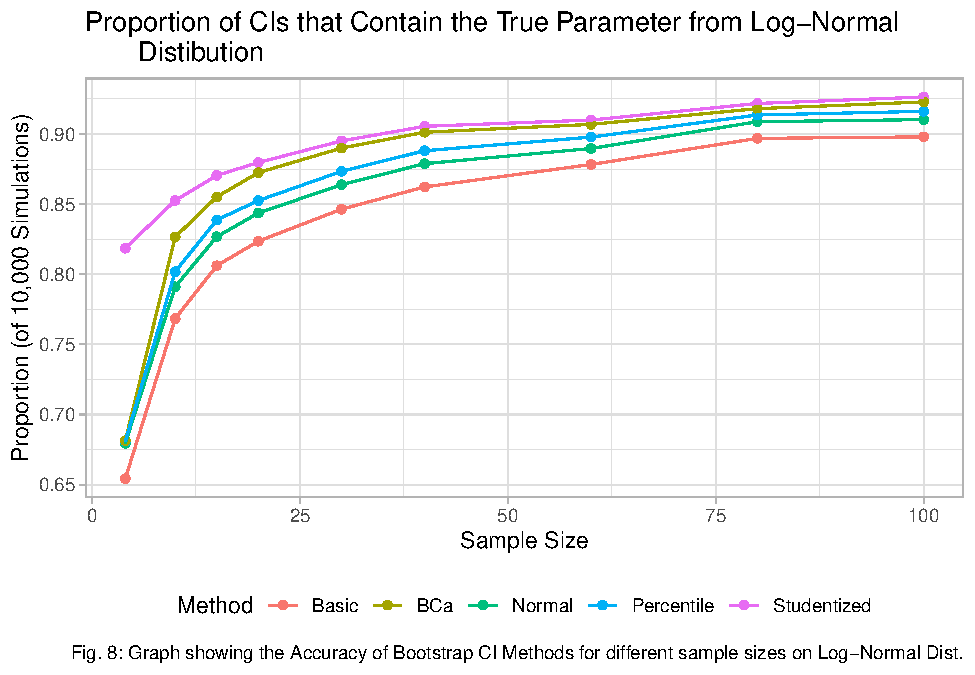
\includegraphics{paper_files/figure-latex/unnamed-chunk-24-1.pdf}

\begin{Shaded}
\begin{Highlighting}[]
\NormalTok{log\_normal\_table}
\end{Highlighting}
\end{Shaded}

\begin{table}

\caption{\label{tab:create graphs}Sampled from Normal Dist.}
\centering
\begin{tabular}[t]{cccccc}
\toprule
Sample Size & Normal & Basic & Studentized & Percentile & BCa\\
\midrule
4 & 0.6795 & 0.6542 & 0.8186 & 0.6810 & 0.6814\\
10 & 0.7911 & 0.7684 & 0.8526 & 0.8019 & 0.8266\\
15 & 0.8268 & 0.8061 & 0.8705 & 0.8387 & 0.8552\\
20 & 0.8437 & 0.8236 & 0.8797 & 0.8526 & 0.8725\\
30 & 0.8639 & 0.8464 & 0.8951 & 0.8734 & 0.8900\\
\addlinespace
40 & 0.8789 & 0.8623 & 0.9055 & 0.8881 & 0.9013\\
60 & 0.8897 & 0.8783 & 0.9100 & 0.8978 & 0.9069\\
80 & 0.9088 & 0.8969 & 0.9218 & 0.9136 & 0.9181\\
100 & 0.9103 & 0.8980 & 0.9264 & 0.9162 & 0.9229\\
\bottomrule
\end{tabular}
\end{table}

\begin{Shaded}
\begin{Highlighting}[]
\NormalTok{normal\_fig}
\end{Highlighting}
\end{Shaded}

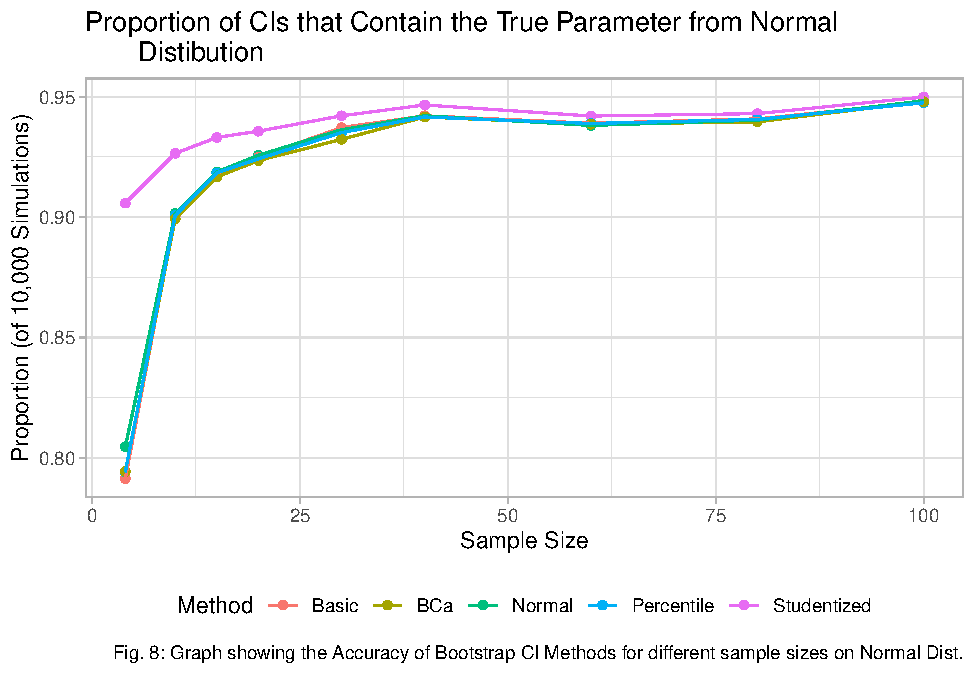
\includegraphics{paper_files/figure-latex/unnamed-chunk-24-2.pdf}

\begin{Shaded}
\begin{Highlighting}[]
\NormalTok{normal\_table}
\end{Highlighting}
\end{Shaded}

\begin{table}

\caption{\label{tab:create graphs}Sampled from Normal Dist.}
\centering
\begin{tabular}[t]{cccccc}
\toprule
Sample Size & Normal & Basic & Studentized & Percentile & BCa\\
\midrule
4 & 0.8046 & 0.7913 & 0.9058 & 0.7941 & 0.7943\\
10 & 0.9015 & 0.9005 & 0.9265 & 0.9007 & 0.8994\\
15 & 0.9187 & 0.9183 & 0.9331 & 0.9184 & 0.9167\\
20 & 0.9257 & 0.9249 & 0.9357 & 0.9242 & 0.9235\\
30 & 0.9363 & 0.9372 & 0.9421 & 0.9351 & 0.9323\\
\addlinespace
40 & 0.9421 & 0.9421 & 0.9466 & 0.9416 & 0.9416\\
60 & 0.9381 & 0.9390 & 0.9420 & 0.9389 & 0.9386\\
80 & 0.9403 & 0.9408 & 0.9430 & 0.9406 & 0.9396\\
100 & 0.9483 & 0.9478 & 0.9499 & 0.9475 & 0.9480\\
\bottomrule
\end{tabular}
\end{table}

\begin{Shaded}
\begin{Highlighting}[]
\NormalTok{gamma\_fig}
\end{Highlighting}
\end{Shaded}

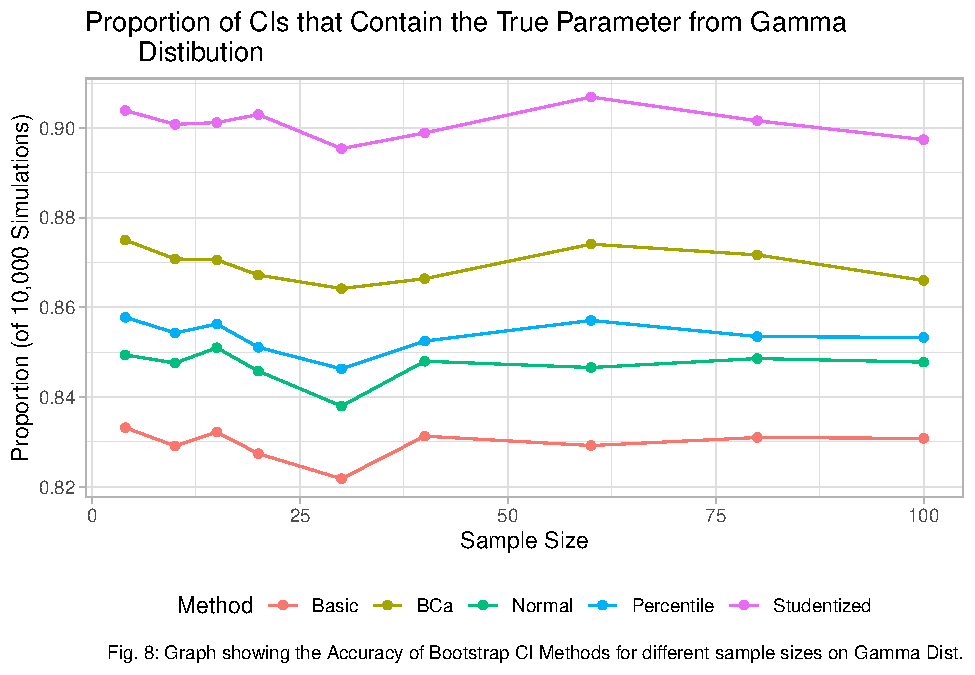
\includegraphics{paper_files/figure-latex/unnamed-chunk-24-3.pdf}

\begin{Shaded}
\begin{Highlighting}[]
\NormalTok{gamma\_table}
\end{Highlighting}
\end{Shaded}

\begin{table}

\caption{\label{tab:create graphs}Sampled From Gamma Dist.}
\centering
\begin{tabular}[t]{cccccc}
\toprule
Sample Size & Normal & Basic & Studentized & Percentile & BCa\\
\midrule
4 & 0.8494 & 0.8332 & 0.9039 & 0.8578 & 0.8750\\
10 & 0.8476 & 0.8291 & 0.9008 & 0.8543 & 0.8708\\
15 & 0.8510 & 0.8322 & 0.9012 & 0.8563 & 0.8706\\
20 & 0.8458 & 0.8274 & 0.9030 & 0.8511 & 0.8672\\
30 & 0.8380 & 0.8218 & 0.8954 & 0.8463 & 0.8642\\
\addlinespace
40 & 0.8480 & 0.8313 & 0.8989 & 0.8525 & 0.8664\\
60 & 0.8466 & 0.8292 & 0.9069 & 0.8571 & 0.8741\\
80 & 0.8486 & 0.8310 & 0.9016 & 0.8535 & 0.8717\\
100 & 0.8478 & 0.8308 & 0.8974 & 0.8533 & 0.8660\\
\bottomrule
\end{tabular}
\end{table}

\begin{Shaded}
\begin{Highlighting}[]
\NormalTok{normal\_df }\OtherTok{\textless{}{-}} \FunctionTok{read.csv}\NormalTok{(}\AttributeTok{file =} \StringTok{\textquotesingle{}normal\_data\_df.csv\textquotesingle{}}\NormalTok{)}

\NormalTok{master\_df\_long }\OtherTok{\textless{}{-}}\NormalTok{ master\_df }\SpecialCharTok{\%\textgreater{}\%}
  \FunctionTok{pivot\_longer}\NormalTok{(}\AttributeTok{cols =} \DecValTok{2}\SpecialCharTok{:}\DecValTok{6}\NormalTok{, }\AttributeTok{names\_to =} \StringTok{"method"}\NormalTok{, }\AttributeTok{values\_to =} \StringTok{"prop"}\NormalTok{) }
    
\NormalTok{master\_fig }\OtherTok{\textless{}{-}} \FunctionTok{ggplot}\NormalTok{(}\AttributeTok{data =}\NormalTok{ master\_df\_long, }
                    \FunctionTok{aes}\NormalTok{(}\AttributeTok{x =}\NormalTok{ Sample\_Size, }\AttributeTok{y =}\NormalTok{ prop, }\AttributeTok{color =}\NormalTok{ method)) }\SpecialCharTok{+} 
  \FunctionTok{geom\_point}\NormalTok{() }\SpecialCharTok{+} \FunctionTok{geom\_line}\NormalTok{() }\SpecialCharTok{+} 
  \FunctionTok{labs}\NormalTok{(}\AttributeTok{title =} \StringTok{"Proportion of CIs that Contain the True Parameter from Log{-}Normal}
\StringTok{       Distibution"}\NormalTok{, }\AttributeTok{x =} \StringTok{"Sample Size"}\NormalTok{, }
       \AttributeTok{y =} \StringTok{"Proportion (of 10,000 Simulations)"}\NormalTok{, }\AttributeTok{color =} \StringTok{"Method"}\NormalTok{,}
       \AttributeTok{caption =} \StringTok{"Fig. 8: Graph showing the Accuracy of Bootstrap CI Methods for different sample sizes on Log{-}Normal Dist."}\NormalTok{) }\SpecialCharTok{+}
  \FunctionTok{theme\_light}\NormalTok{() }\SpecialCharTok{+}
  \FunctionTok{theme}\NormalTok{(}\AttributeTok{legend.position=}\StringTok{"bottom"}\NormalTok{)}

\NormalTok{master\_fig}
\end{Highlighting}
\end{Shaded}


\bibliographystyle{agsm}
\bibliography{bibliography.bib}


\end{document}
